
%% include the next line for the long version of the paper
\newcommand{\longpaper}{}



\newcommand{\draftpaper}{}
\newcommand{\revision}{}

\emergencystretch=\hsize
\lefthyphenmin=2
\righthyphenmin=2
\tolerance=9999

% detect interpreter: pdflatex or latex

\newif\ifpdf
\ifx\pdfoutput\undefined
  \pdffalse
\else
  \pdftrue
\fi

\newif\iflong
\ifx\longpaper\undefined
  \longfalse
\else
  \longtrue
\fi

\newif\ifdraft
\ifx\draftpaper\undefined
  \draftfalse
\else
  \drafttrue
\fi

\newif\ifverbose
\ifx\verbosepaper\undefined
  \verbosefalse
\else
  \verbosetrue
\fi

%
% REVCHANGE
%
\newif\ifrev
\ifx\revision\undefined
  \revfalse
\else
  \revtrue
\fi

% use document class IROS with any paper size:

%%\iflong
%%  \documentclass[a4]{epirob}
  \documentclass[]{article}
%%\else
%%  \documentclass[a4paper]{IROS}
%%\fi

	 \usepackage{fancyhdr}
	 \usepackage{fullpage}

\lhead[\fancyplain{}{}]       {\fancyplain{}{}}
\rhead[\fancyplain{}{\thepage}]       {\fancyplain{}{\thepage}}
\renewcommand{\headrulewidth}{0pt}
%
%	\addtolength{\oddsidemargin}{-.875in}
%	\addtolength{\evensidemargin}{-.875in}
%	\addtolength{\textwidth}{1.75in}

%	\addtolength{\topmargin}{-.875in}
%	\addtolength{\textheight}{1.75in}

\usepackage{pf-mod}

\usepackage{natbib}

\usepackage[nolists,tablesfirst]{endfloat}


\renewcommand{\cite}{\citep}


%%\documentclass[a4paper]{article}

%%\documentstyle{doublespace}



\ifpdf
  \usepackage{graphicx}
\else
  \usepackage[dvips]{graphicx}
\fi

\usepackage{psfig}

%%\setlength{\baselinestretch}{1.62}

%5\usepackage{setspace}
%%\setstretch{2.0}
\usepackage{doublespace}

\usepackage{pf-mod}

%\let\Caption\caption
%\renewcommand\caption[1]{%
%    \Caption[#1]{}%
%}

\begin{document} 



\onecolumn


% create the title header:
\ifrev
\title{Better Vision Through Manipulation}
\else
\title{Early Integration of Vision and Manipulation}
\fi

\author{
Giorgio Metta\\
LIRA-Lab, DIST\\
University of Genova\\
Genova, Italy\\
{\tt pasa@dist.unige.it}
\and 
Paul Fitzpatrick\\
Artifical Intelligence Lab\\
Massachusetts Institute of Technology\\
Cambridge, MA, USA\\
{\tt paulfitz@ai.mit.edu}
}

%%\iflong
%%  \author{Giorgio Metta$^{*,**}$
%%        \and
%%         Paul Fitzpatrick$^{**}$}
%%  \affiliation{\rm $^{*}$LIRA-Lab, DIST \\
 %%              University of Genova \\
 %%               Viale F. Causa, 13 \\
  %%              16145 Genova, Italy \\
  %%         \and
 %%             $^{**}$MIT AI Lab\\
 %%            200 Technology Square \\
 %%            Cambridge, MA 02139 US }
%%\else
%%\author{Paul M. Fitzpatrick$^{*}$ and Giorgio Metta$^{*,\dagger}$}
%%\affiliation{
%%$^{*}$MIT AI Lab -- Massachussetts Institute of Technology -- USA\\
%%$^{\dagger}$Lira Lab, DIST -- University of Genova -- Italy
%%}
%%\fi

%%\maketitle\thispagestyle{empty} % don't forget \thispagestyle{empty}, otherwise you'll get page numbering


\faketitle\thispagestyle{empty}

\vskip 3em%

\begin{center}
Address correspondence to Giorgio Metta, LIRA-Lab, DIST, Viale Causa, 13 -- I-16145 Genova, Italy 

(phone: +39 0103532791, fax: +39 0103532948).
\end{center}

\clearpage

\thispagestyle{empty}

{
\newcommand{\shorten}{use this option to shorten the abstract (200 words max)}


We describe YARP, Yet Another Robot Platform, an open-source project
that encapsulates lessons from our experience in building humanoid
robots.  The goal of YARP is to minimize the effort
devoted to infrastructure-level software development
 by facilitating code reuse, 
modularity and so maximize research-level development and collaboration. Humanoid robotics is a ``bleeding edge'' field of research, with constant flux in sensors, actuators, and 
processors.  Code reuse and maintenance is therefore a significant 
challenge. We describe the main problems we faced and the 
solutions we adopted. 
In short, the main features of YARP include support for inter-process
communication, image processing as well as a class hierarchy
to ease code reuse across different hardware platforms. YARP
is currently used and tested on Windows, Linux and QNX6 which are common 
operating systems used in robotics. 

%With YARP, we lay the ground-work for long-term
%software development. [need to review this]


\begin{center}
{\bf keywords: } humanoid robotics, active segmentation, epigenesis
\end{center}

\begin{center}
{\bf running title: } Vision and Manipulation
\end{center}

}




\clearpage


\maketitle

\ifdraft
  \pagenumbering{arabic}
  \thispagestyle{plain}
  \pagestyle{plain}
\fi

\pagestyle{fancy}

% write the abstract with the Abstract-environment:

We describe YARP, Yet Another Robot Platform, an open-source project
that encapsulates lessons from our experience in building humanoid
robots.  The goal of YARP is to minimize the effort
devoted to infrastructure-level software development
 by facilitating code reuse, 
modularity and so maximize research-level development and collaboration. Humanoid robotics is a ``bleeding edge'' field of research, with constant flux in sensors, actuators, and 
processors.  Code reuse and maintenance is therefore a significant 
challenge. We describe the main problems we faced and the 
solutions we adopted. 
In short, the main features of YARP include support for inter-process
communication, image processing as well as a class hierarchy
to ease code reuse across different hardware platforms. YARP
is currently used and tested on Windows, Linux and QNX6 which are common 
operating systems used in robotics. 

%With YARP, we lay the ground-work for long-term
%software development. [need to review this]


% ...and start writing!


\section{Introduction}

YARP is written by and for researchers in humanoid robotics, who find
themselves with a complicated pile of hardware to control with an
equally complicated pile of software.

%YARP includes modules to facilitate software development on
%humanoid robots, including abstractions for the operating system,
%image processing, physical devices, mathematical operations, etc.
%
At the time of writing, running decent visual, auditory, and tactile
perception while performing elaborate motor control in real-time
requires a lot of processor cycles. The only practical way to get
those cycles at the moment is to have a cluster of computers. Every
year what one machine can do grows, but so also do our demands~--
humanoid robots stretch the limits of current technology, and are
likely to do so for the foreseeable future.
Moreover, software is in general tight to the hardware on which it runs.
This limits modularity and code reuse which, in turn, complicates software 
development and mantainability. In the last few years we have been developing
a software platform to ease these tasks and improve the software quality on 
our robotic platforms. 
We want to reduce the effort devoted to programming to increase the 
time spent doing research. At the same time, we would like to have 
stable robotic platforms to work with.
Today YARP is a platform for long-term software 
development for applications that are real-time, computation-intensive, 
and involve interfacing with diverse and changing hardware. It is is 
successfully used on several platforms in our research Laboratories. 
The diversity of contexts on which it has been applied
show that our efforts have been somehow successful [reference table?].


\begin{table}
\centerline{\small
\begin{tabular}{|l|c|c|c|}
\hline
Robot&Laboratory&size&OS\\
\hline
Babybot&LIRA-Lab&13&Win/QNX6\\
Eurobot&LIRA-Lab&11&Win/QNX6\\
RobotCub&LIRA-Lab&3&Win\\
Obrero&MIT-CSAIL&4&Linux/OSX\\
Mertz&MIT-CSAIL&4&Linux\\
Domo&MIT-CSAIL&6&Linux\\
COG&MIT-AILab&30&QNX4/Linux\\
Kismet&MIT-AILab&12&Linux/Win/QNX4\\
\hline
\end{tabular}
}
\caption {
Robots using YARP.
}
\end{table}


\section{Motivation}

Let us now introduce the main features of YARP by describing the general lessons
we have learned and applied to YARP.
%
%
%Here are some general lessons we have learned, and apply to YARP.
%
%\begin{itemize} \pflist
%\item {\bf One processor is never enough.}

\textit{\textbf{One processor is never enough.}}
Designing a robot control system as a set of processes running on a
set of computers is a good way to work. It minimizes time spent wrestling with
code optimization, rewriting other people's code, and maximizes
time spent actually doing research.  The heart of YARP is a
communications mechanism to make writing and running such processes as
easy as possible. Even where mobility is required this is not a limiting
factor if teathers or wireless communication are practical.

%\item {\bf Modularity.} 
\textit{\textbf{Modularity.}}
Code is better maintainaed and reused if it is organized in small processes 
each one performing a simple task. In a cluster of computers some processes 
are bound to specific machines (usually when they require particular hardware 
device), but most of the times they can run on any of the available computers. 
With YARP it is easy to write processes that are location independent and 
that can run on different machines without code changes. This allows to move 
processes across the cluster at runtime to redistribute the computational 
load on the CPUs or to recover from a hardware failure. 
YARP does not contain any means of automatically allocating processes as in 
some approaches like GRID \cite{grid}. Our apporach is that of leaving this
task to the user to act sensibly and allocate the processes. The rationale is that: i)
special interface hardware is necessarily to be controlled by the appropriate piece of 
software, and ii) in an etherogeneous network of processors, faster processors might 
need to be allocated differently from slower processors. The final behavior is that of 
a sort of ``soft real-time'' parallel computation cluster without the more demanding
requirements of a real-time operating system.

\textit{\textbf{Minimal interference.}}
%Ports were designed with the two-fold goal of reducing the interactions at large between 
%the various components of the robot controller and, simultaneously, to allow efficient 
%communication between interacting parts of the system. The bottleneck in this approach
%would eventually be the available bandwidth on the network. 
As long as enough resources are available, the addition of new components 
should minimally interfere with existing processes. This is important, since often 
the actual performance of a robotic controller depends on the timing of various signals. 
While this is not strictly guaranteed by the YARP infrastructure, the problem is in 
practice alleviated computationally by allowing the inclusion of more processors to 
the network, and from the communication point of view by the buffer policy.
%isolating sub-components.

%\item {\bf Stopping hurts.}
\textit{\textbf{Stopping hurts.}}
It is a commonplace that human cycles are much, much more expensive
than machine cycles.  In robotics, it turns out that the human
cost of stopping and restarting a process can be very high.
For example, that process may interface with some
custom hardware which requires a physical reset.  
That reset many need to be carefully ordered with respect to when the
process is stopped and started.
%
There may be other dependent processes that need to be restarted in
turn, and other dependent hardware. 
%
%
%
These ordering constraints are time-consuming to satisfy.
%
YARP does its part to minimize dependencies between processes,
% so only true physically required dependencies remain.  
communication channels between processes can come and go. 
A process that is killed or dies
unexpectedly does not require processes to which it connects to be
restarted. This also simplify cooperation between people, as
it minimizes the need to synchronize development on different  
parts of the system.
%
%In complex systems, with dozens of processes and hundreds of connections, it might become
%unpractical to shut down and restart the whole system every time a module is even slightly 
%changed. YARP allowing the run-time connection of channels permits the disconnection of 
%only those parts of the system that need to be, for instance, rebuilt. 
%
%\item {\bf Humility helps.}

\textit{\textbf{Humility helps.}}
Over time, sofware for a sophisticated robot needs to 
aggregate code written by many different people in many
different contexts.  Doubtless that code will have
dependencies on various communication, image processing,
and other libraries. Very often the operating system on which
software is developed pose similar constraints. This is especially
true with code that relies heavily on the services offered by the 
operating system (such as communication, scheduling, synchronization primitives, 
and device driver interface).
%
Any component that tries to place itself ``in control'' and has strong
constraints on what dependencies are permissible will not be tolerated
for long.  It certainly cannot co-exist with another component
with the same assumption of ``dominance''. 
Although YARP offers support for communication, image processing,
interfacing to hardware etc., it is written with an {\em open world}
mindset.  We do not assume it will be the only library used, and
endeavor to be as friendly to other libraries as possible.
%
YARP allows interconnecting many modules seamlessly without subscribing
to any specific programming style, language interface, 
or demanding specifications as for instance in CORBA~\cite{vinoski97corba}
or DCOM~\cite{dcom}. Such systems, although far more powerful than YARP,
require a much tighter link between the general algorithmic code and the 
communication layer.
We have taken a more lightweight approach: YARP is a plain library linked
to uses-level code that can be used directly just by instantiating appropriate classes.
%
% and communication does not require any diversion
% of pre-existing threads. That is, YARP is a plain library linked to user-level
% code and as such migration to YARP can be easily carried out a posteriori. 
%
% Systems such as CORBA~\cite{vinoski97corba}, although far more powerful than YARP, require 
%
% adhering to well-defined interface specificiations (nothing bad as such) but consequently 
%
% a much tighter link between the general algorithmic code and the communication layer.
%
% is much 
% stricter. 
%
%
%
Finally, other programming languages can access YARP as well, provided they
have means of linking and calling C++ code. We have successfully used
YARP from within Matlab or L~\cite{brooks90behavior}.

%It is userful to reserve
%that role for the occasional poorly-designed hardware device that
%assumes it is the center of the universe.

%\end{itemize}

\noindent
%
%The OS library contains the communication facilities described in
%section \ref{sec:communication} and classes implementing
%synchronization routines (like mutexes and semaphores) and
%threads. 
%
\textit{\textbf{Exploit diversity.}}
%
Different operating systems offer different
features. Sometimes it is easier to write code to perform a given task
on a platform as opposed to another. This can happen for example if 
device drivers for a given board are provided only on a specific platform or
if an algorithm is available open source on another. We decided to reduce the
dependencies with the operating system. For this we
use ACE~\cite{ACEBook}, an open source library providing a framework for
concurrent programming across a very wide range of operating
systems. YARP inherits the portability of ACE and has indeed been used and
tested on Windows, Linux and QNX 6.



YARP's core communication model was the survivor from an early humanoid robot
controlled by a set of Motorola 68332 processors, an Apple Mac, and a loose network
of PCs running QNX, Linux, and Microsoft Windows.  Communication was a
hodge-podge of dual-port RAM, QNX message passing, CORBA, and raw
sockets.  At one point, three incompatible communication protocols
layered over QNX message passing were in use simultaneously.  This
variety was a consequence of organic growth, as developers added new
modules to the robot.  YARP began as one of the communication
protocols built on QNX message passing.  A key, defining, feature of
YARP was that it was {\em broad-minded}: it was
implemented in the form of a library which placed minimal constraints
on user code; communication resources did not need to be allocated at
any particular time or place in a program; reading messages could be
blocking, polling, or callback based, etc. This meant it could be
easily added without disturbing existing code, and communication could
be moved across to the new protocol piece by piece.

%The basic YARP module is an IPC infrastructure that supports communication across a
%network exploiting different protocols. 
%

%The mathematical library provides classes and functions to handle
%vectors and matrices, together with a few algebraic routines like
%single value decomposition, QR and LU factorization.

%More details about the image processing library and the device driver
%library can be found in the next sections.



\section{The experimental platform}

This work is implemented on the robot Cog, an upper torso humanoid
\ifrev
\cite{brooks99cog, group-IEEE-2000}.  The robot has previously been applied to tasks
\else
\cite{brooks99cog}.  The robot has previously been applied to tasks
\fi
such as visually-guided pointing \cite{Marjanovic-96-SAB}, and
rhythmic operations such as turning a crank or driving a slinky
\cite{williamson98neural}.  Cog has two arms, each of which has six
degrees of freedom -- two per shoulder, elbow, and wrist.  The joints
are driven by series elastic actuators \cite{williamson95series} --
essentially a motor connected to its load via a spring (think strong
and torsional rather than loosely coiled).  The arm is not designed to
enact trajectories with high fidelity.  For that a very stiff arm is
preferable.  Rather, it is designed to perform well when interacting
with a poorly characterized environment, where collisions are frequent
and informative events.

\begin{figure}[tbh]
\centerline{
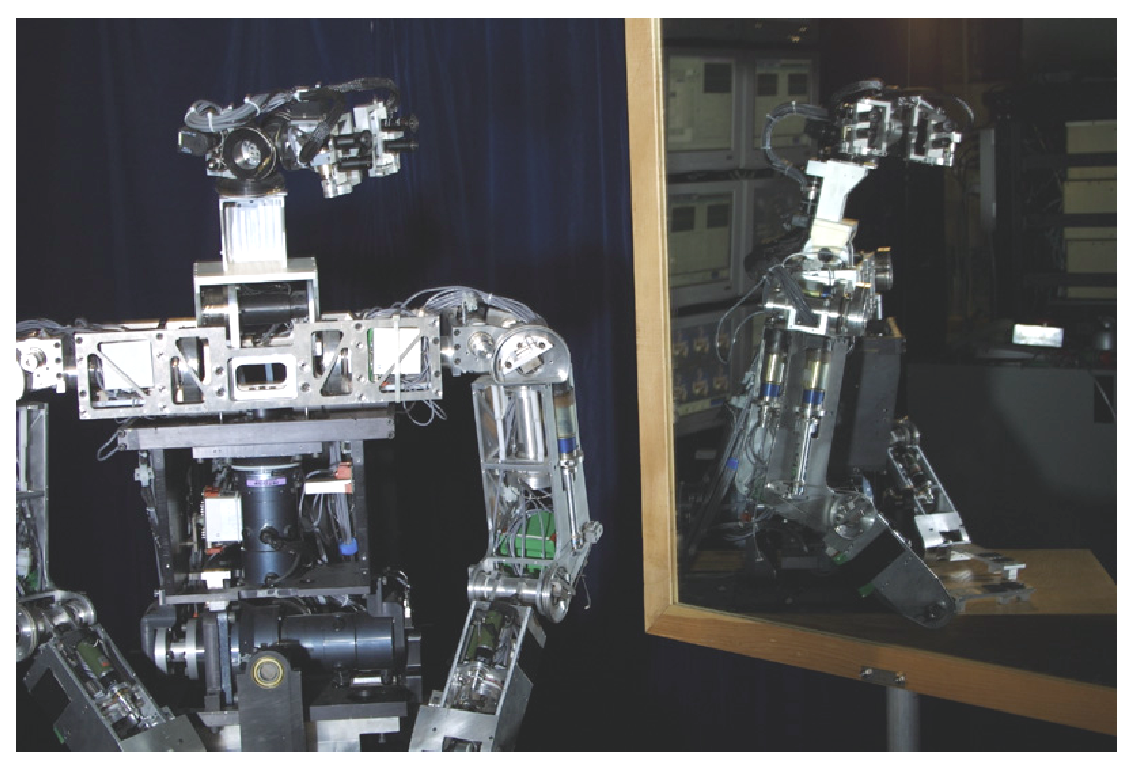
\includegraphics[width=12cm]{mirror-cog.eps}
%%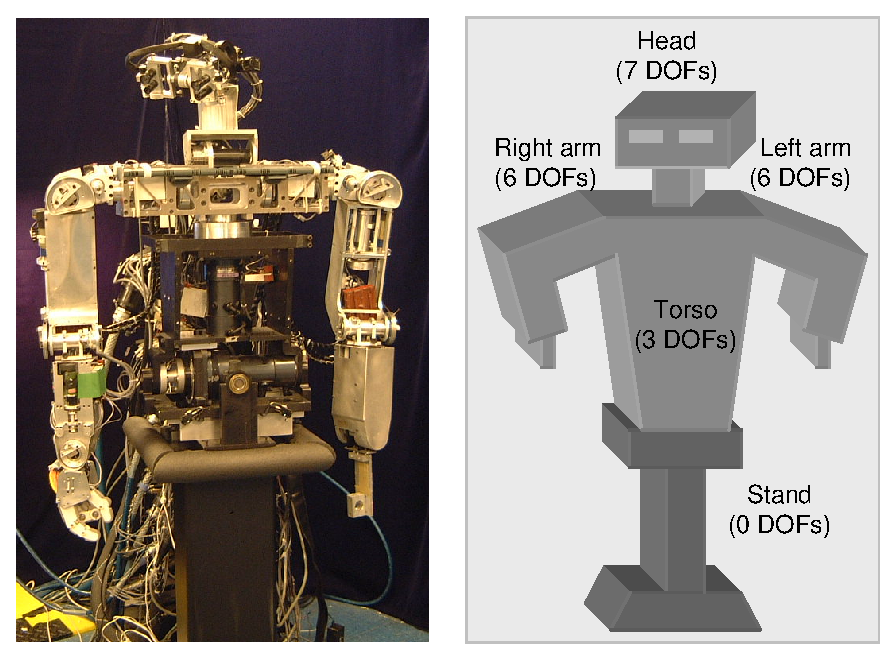
\includegraphics[width=12cm]{cog-schematic.eps}
%%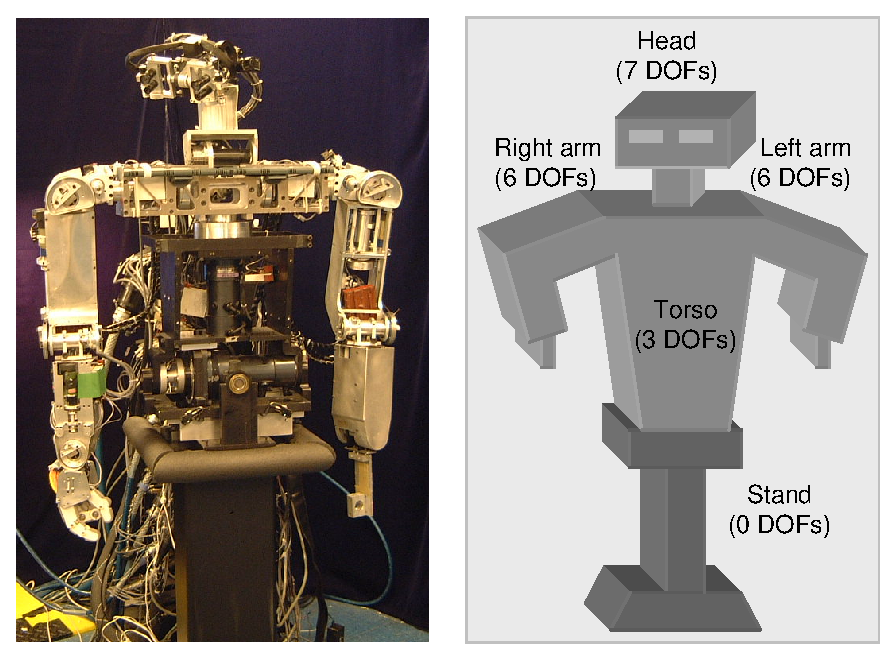
\psfig{file=cog-schematic.eps,height=2.5in,clip=,silent=}
}
\caption{ 
%
  The robot Cog, an upper-torso humanoid.  
The ultimate goal of this work is for our robot to follow chains of
causation outwards from its own simple body into the complex world.
Such an incremental process suggests that perception and action
develop together, supporting each other.
%The arms terminate
%  either in a primitive ``flipper'' or a four-fingered hand.  
% Degrees of freedom (DOFs) of the robot Cog.  The arms terminate
% either in a primitive ``flipper'' or a four-fingered hand.  
\ifverbose
The hand
  is an independent research project by Matthew Marjanovi\'{c}, and
  will not be employed or described here.  
\fi
  The head, torso, and arms
  together contain 22 degrees of freedom.
%
}
\label{fig:cog-schematic}
\end{figure}


\ifverbose
\begin{figure}[tbh]
\begin{center}
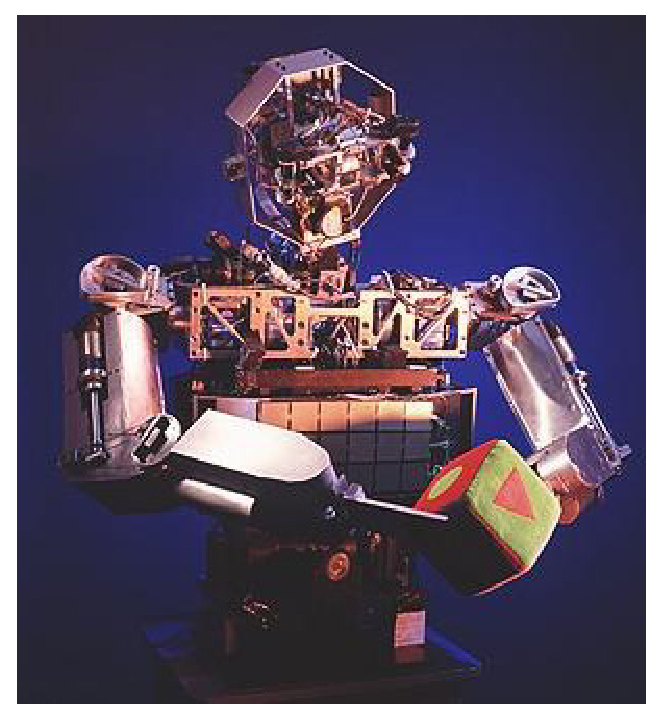
\includegraphics[height=3.5cm]{cog5-flip.eps}
\ \ \ \ 
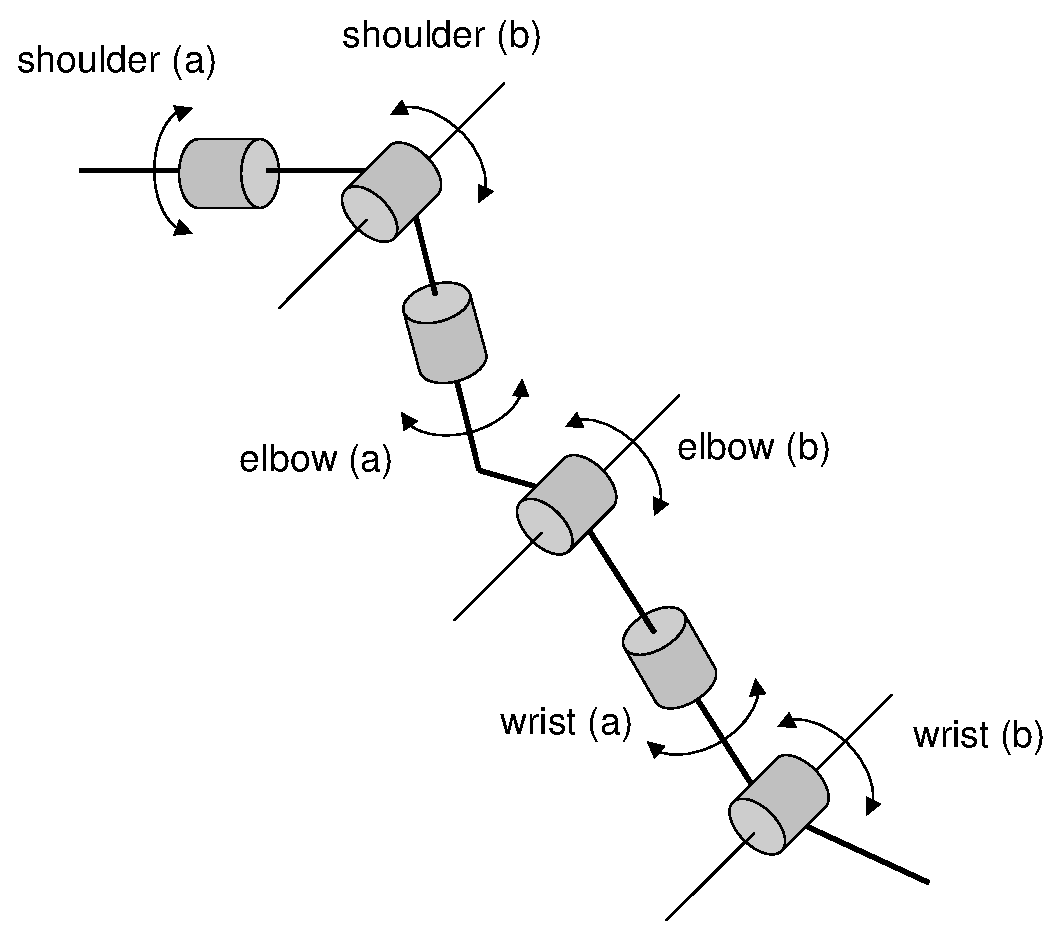
\includegraphics[height=3.5cm]{arm-motors.eps}
\caption{ 
\label{fig:arm-motors}
%
Kinematics of the arm, following \protect\cite{williamson99robot}.
There are a total of six joints, divided into a pair for each of
the shoulder, elbow, and wrist/flipper.
%
}
\end{center}
\end{figure}
\fi

\ifrev
The following sections \ref{sec:directeffect} through \ref{sect:recognition} 
explore the four levels of causation which are at the core of 
our working hypothesis. The rationale of the experiments is to show
that one possible route to object recognition goes through the
``understanding'' of longer chains of cause-effects relationships.
In particular section \ref{sec:directeffect} describes the simplest causal
chain where motion of the robot causes immediate visual effects. Simple
cross-correlation over time of motor and visual signals allows localizing
the robot's end-point. Reaching is seen as an extension of the same
mechanism. 
Subsequently, we show in section \ref{sec:poking} how the robot 
explores its peripersonal space and get to explore physical objects.
Exploiting causality in this case leads to object segmentation 
(figure/ground separation). In this case there is a potentially
delayed effect because initiating the reaching action does not
automatically lead to poking.
The experiments described in section \ref{sect:experiment} and 
\ref {sec:mirror} build on top of the segmentation to learn object 
``affordances''. Exploring further a complex causal chain where
the actions of others are considered moves us naturally to 
a ``mirror neuron'' like response.
Eventually object recognition is presented in section \ref{sect:recognition}
as a combination of affordances and the acquisition of data 
through multiple instances of the same manipulative act.
\fi


\section{Perceiving the body in action}

Motion of the arm may generate optic flow directly through the
changing projection of the arm itself, or indirectly through an object
that the arm is in contact with.  While the relationship between the
optic flow and the physical motion is likely to be complex,
the correlation in time of the two events should be
exceedingly precise.  This time-correlation can be used as a
``signature'' to identify parts of the scene that are being influenced
by the robot's motion, even in the presence of other distracting
motion sources.  In this section, we show how this tight correlation
can be used to local\ize{} the arm in the image without any prior
information about visual appearance.  
%%In the next section we will show
%%that once the arm has been localized we can go further, and identify
%%the boundaries of objects with which the arm comes into contact.

\subsubsection*{Reaching out}

The first step towards manipulation is to reach objects within the
workspace.  If we assume targets are chosen visually, then ideally we
need to also locate the end-effector visually to generate an error
signal for closed-loop control.  Some element of open-loop control is
necessary since the end-point may not always be in the field of view
(for example, when it is in its resting position), and the overall
reaching operation can be made faster with a feed-forward contribution
to the control.

\begin{figure}[tb]
\begin{center}
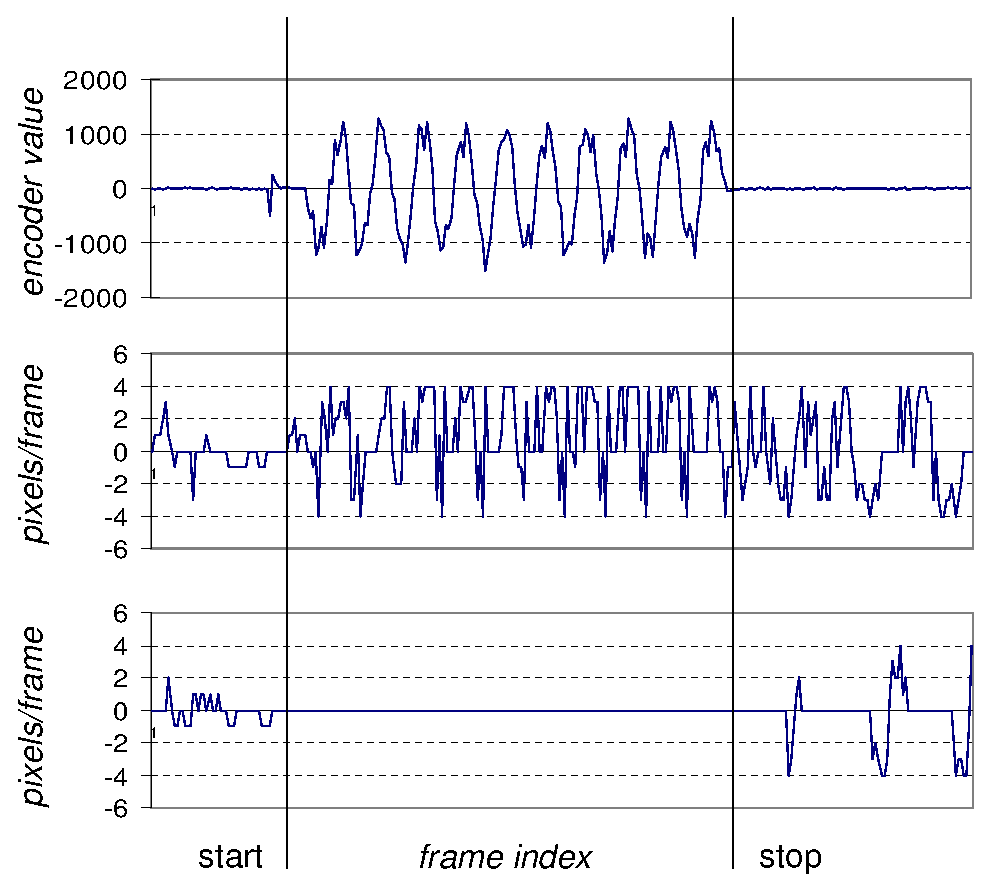
\includegraphics[width=6.0cm]{joint-correlation3.eps}
%%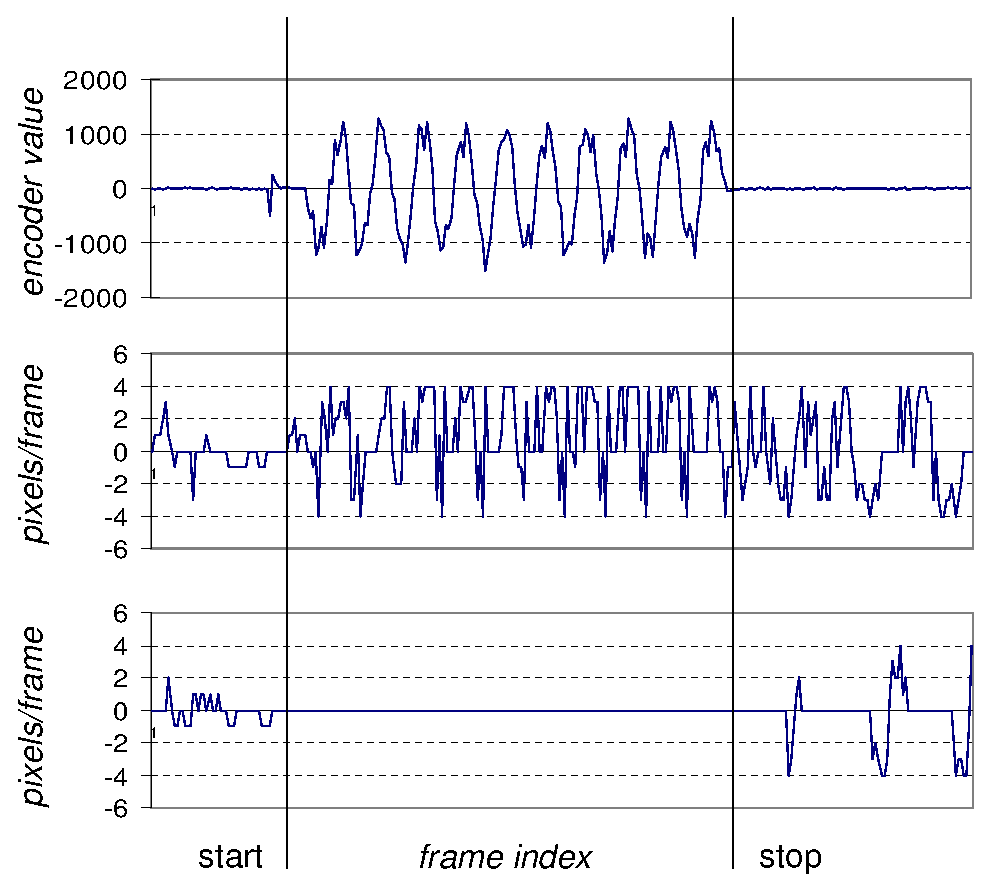
\includegraphics[width=\columnwidth]{joint-correlation3.eps}
\caption{ 
\label{fig:joint-correlation}
%
An example of the correlation between optic flow and arm movement.
The traces show the movement of the wrist joint (upper plot)
and optic flow sampled on the arm (middle plot) and away from it (lower
plot).  As the arm generates a repetitive movement, the oscillation
is clearly visible in the middle plot and absent in the lower.
Before and after the movement the head is free to saccade, generating the
other spikes seen in the optic flow.
%
}
\end{center}
\end{figure}


The simplest possible open loop control would map directly from a
fixation point to the arm motor commands needed to reach that point
\cite{metta99developmental} using a stereotyped trajectory, perhaps
using postural primitives \cite{mussa-ivaldi92vector}.  If we can
fixate the end-effector, then it is possible to learn this map by
exploring different combinations of direction of gaze vs.  arm
position \cite{Marjanovic-96-SAB,metta99developmental}.  So locating
the end-effector visually is key both to closed-loop control, and to
training up a feed-forward path.  We shall demonstrate that this
local\iz{}ation can be performed without knowledge of the arm's appearance,
and without assuming that the arm is the only moving object in the
scene.

\ifverbose
NEW The closed loop control requires the identification of both the
end-effector and the target in the image plane. As in the visual
servoing literature \cite{espiau92new} it is certainly possible to
design a feedback controller based on the knowledge of the Jacobian
mapping between the image and the robot joint space -- globally
represented by both the position of the cameras in space and the arm.
The state space in our case is 13-dimensional. Constructing the
Jacobian requires the calibration of the robot and the estimation of
the kinematics.  On the other hand, for the configurations where the
object and the end-point are close one to the other, it is possible to
simplify the formulation by assuming the controller is locally
constant with respect to the arm position (this removes 6 dimensions).
Still the controller is a function of the configuration of the head.
This dependency must be roughly taken into account to move the arm
correctly. The requirements in terms of precision are in fact not that
stringent because what matters for the closed loop controller is that
the sign remains negative with respect to the visual error. For our
purpose this relationship can be learned by the same exploration
procedure mentioned above for the open loop controller.  For both
controllers the problem translates into local\iz{}ing the arm's end-point
in the image plane. We shall demonstrate that visual local\iz{}ation can
be performed without relying on a particular \ahhcolor{} or pattern but
simply on movement and motor information.
\fi

\begin{figure}[tb]
\begin{center}
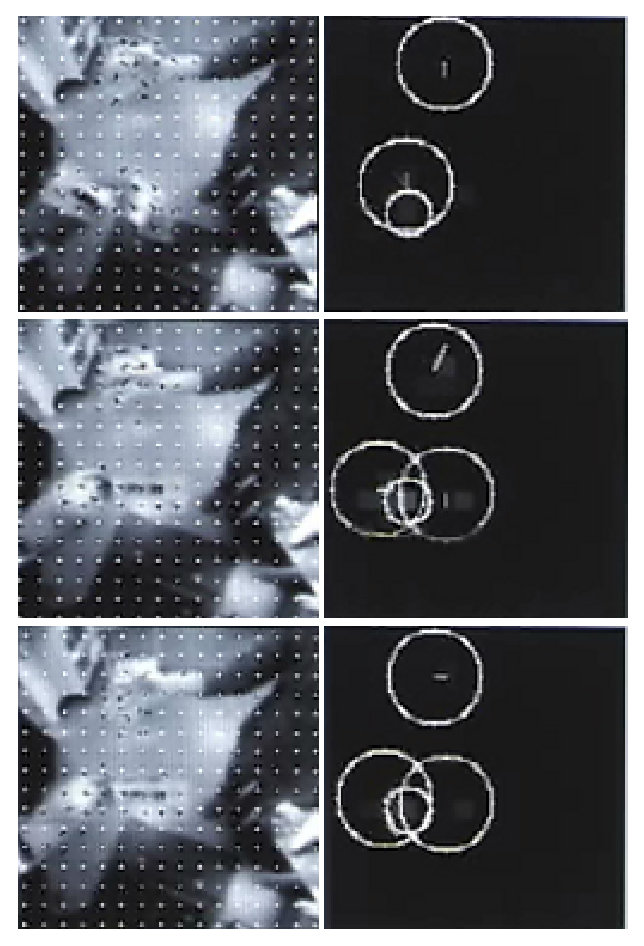
\includegraphics[width=5cm]{arm-detection2.eps}
\caption{ 
\label{fig:arm-detection}
%
Detecting the arm/gripper through motion correlation. The robot's
point of view and the optic flow generated are shown on the left. On
the right are the results of correlation.  Large circles represent the
results of applying a region growing procedure to the optic flow.
Here the flow corresponds to the robot's arm and the experimenter's
hand in the background. The small circle marks the point of maximum 
correlation, identifying the regions that correspond to the robot's own arm.
%
}
\end{center}
\end{figure}


\subsubsection*{Local\iz{}ing the arm visually}

The robot is not a passive observer of its arm, but rather the
initiator of its movement.  This can be used to distinguish the arm
from parts of the environment that are more weakly affected by the
robot.  The arm of a robot was detected in \cite{Marjanovic-96-SAB} by
simply waving it and assuming it was the only moving object in the
scene.  We take a similar approach here, but use a more
stringent test of looking for optic flow that is correlated with
the motor commands to the arm.  This allows unrelated movement
to be ignored.  Even if a capricious engineer were to 
replace the robot's arm with one of a very different appearance,
and then stand around waving the old arm, this detection method
will not be fooled.  

The actual relationship between arm movements and the optic flow they
generate is complex.  Since the robot is in control of the arm, it can
choose to move it in a way that bypasses this complexity.  In
particular, if the arm rapidly reverses direction, the optic flow at
that instant will change in sign, giving a tight, clean temporal
correlation.  Since our optic flow processing is coarse (a $16\times
16$ grid over a $128\times 128$ image at 15 Hz), we simply repeat this
reversal a number of times to get a strong correlation signal during
training.  With each reversal the probability of correlating with
unrelated motion in the environment goes down.  
%%This probability could
%%also be reduced by higher resolution (particularly in time) visual
%%processing.

\ifverbose
Local\iz{}ing the robot arm is not the same as searching into the visual
space for a generic object we do not have any expectancy on its
whereabouts. The robot can exploit the fact it looks for its own body
part to self-generate useful cues to help the local\iz{}ation. The
fundamental idea is to cross-correlate the presence of motion in the
image with the actual arm motion as sensed through proprioception (or
efference copy). When the two quantities have a positive correlation
over a given time window, we can assert that that image location
belongs to the visual projection of the arm. From the visual point of
view, the optic flow can be used. We employed a block matching
technique over a 16x16 grid out of a 128x128 pixels image.
\fi


\ifverbose
\begin{figure}[tb]
\begin{center}
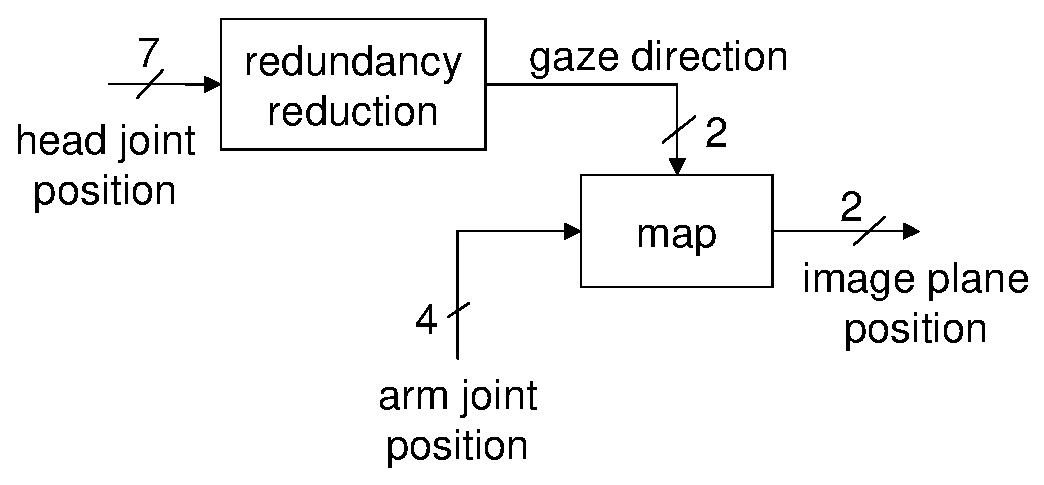
\includegraphics[width=\columnwidth]{mapping-reach.eps}
\caption{ 
\label{fig:mapping-reach}
%
Mapping from proprioceptive input to a visual prediction. Head and arm
joint positions are used to estimate the position of the projection of
the hand in the image plane.  Redundant configurations of the (7 DOF)
head are mapped to a simpler (2D) representation, and the wrist-related 
DOFs of the arm are ignored.
%
}
\end{center}
\end{figure}
\fi

\ifverbose
These two ideas were exploited contextually. The cross-correlation
runs on a 500ms time window while the robot generates a relatively
high-frequency movement. The resulting correlation array (each pixel
is correlated with all joints) is post-processed by a thresholding
procedure and subsequently by a region-growing algorithm. Regions are
identified and labeled. The arm position is identified as the \ahhcenter{}
of mass of the region containing the maximum of the correlation
function.
\fi

Figure~\ref{fig:joint-correlation} shows an example of this procedure
in operation, comparing the velocity of the arm's wrist with the optic
flow at two positions in the image plane.  A trace taken from a
position away from the arm shows no correlation, while conversely the
flow at a position on the wrist is strongly different from zero over
the same period of time.  Figure~\ref{fig:arm-detection} shows
examples of detection of the arm and rejection of a distractor.


\subsubsection*{Local\iz{}ing the arm using proprioception}

The local\iz{}ation method for the arm described so far relies on a
relatively long ``signature'' movement that would slow down reaching.
This can be overcome by training up a function to estimate the
location of the arm in the image plane from proprioceptive information
(joint angles) during an exploratory phase, and using that to 
constrain arm local\iz{}ation during actual operation.
%%As a function approximator we simply fill a look-up table,
%%reducing the 11-dimensional input space of joint angles based on 
%%the much lower number of degrees of freedom used in controlling them
%%(see Figure~\ref{fig:mapping-reach}).
Figure~\ref{fig:predict-position} shows the resulting \ahhbehavior{}
after about twenty minutes of real-time learning. 
%
\ifverbose
Note as both the
position of the arm and the direction of gaze change in these
examples: the position of objects such as the base of the robot at the
bottom of the image varies.
\fi
%
\ifverbose
We can imagine building a function from examples to predict the
position of the arm/end-point in the image plane. Examples are
collected when the arm is local\iz{}ed and have the form of joint
space-image coordinates [equation here?]. In principle a very big
lookup table can be used. The problem is that the input space is
13-dimensional (7 degrees of freedom describing the head configuration
and 6 describing the arm position), and nearest neighbor lookup tables
are known to work poorly in highly dimensional spaces. Beside,
collecting enough samples to span the space densely enough might
require a very long time. We can observe though that only the first
four arm joints determine the appearance of the end-point in the image
plane (the wrist is irrelevant), and the position in space of the
image plane although determined by the head configuration can be
described by only two numbers. These two parameters describe only the
orientation and not the position in space. In theory a distance factor
should be also considered, but it would only marginally influence the
map because the change in distance of the arm with respect to the
camera is small for the allowed movement of the head/arm [hope I
convinced the audience].
\fi


\ifverbose
Can we determine which is the set of redundant configuration of the
head for each given orientation of the camera? We can indeed spot when
two orientations of the camera are the same in spite of the head
configuration been different: this is true if the following statements
are true:
%
\begin{itemize}
%
\item Projection of the arm end-point in the image plane.
%
\item Arm joint position.
%
\item The head configurations are different.
%
\end{itemize}
%
Whenever a new data point (input/output) is used for training, it is
checked against all existing elements in the lookup table. If any of
them satisfy the above-mentioned conditions it is not inserted as a
new point but rather as belonging to the same camera direction.
Figure~\ref{fig:mapping-reach} depicts a schematic of the map as
implemented.

\fi

\ifverbose
\section{Putting things together}

Figure 6 shows how all components of the reaching subsystem are put
together. The lowest level controller is a double loop consisting of a
torque loop based on the reading of the joint strain gauges, and a
position/velocity feedback loop based on the potentiometer readings.
Depending on the tuning of the position/velocity gain it is possible
to obtain a low stiffness yet precise enough controller. Our tuning in
fact has a low positional gain and a relatively higher velocity gain.
The \ahhbehavior{} is thus that of a low-stiffness controller with still a
good \ahhbehavior{} when closing a velocity loop [unclear].

The successive level above is a simple linear combination of postural
primitives. There are four primitives in the present implementation,
which span a good portion of the arm workspace frontal to the robot
chest. Primitives are defined in joint space.

Oscillatory movements are generated by a specific subsystem in
parallel to the postural primitives block. Oscillations are created by
specifying directly the speed of the arm joints.

Further up in the control chain there is the open loop controller.
This is implemented as a nearest neighbor lookup table mapping the
gaze direction into a set of coefficient. The coefficients are the
weights of the linear combination of postural primitives.

The arm locator algorithms control in different ways both the
generation of appropriate movements for the self-local\iz{}ation and the
switching between different control regimes (not indicated in figure).

There are two caveats: first, an additional and more precise visual
bit of information is probably needed, and second, the closed loop
controller has not been implemented yet. The former issue can probably
be solved by looking for a gray blob close to the predicted arm
position. Once the position of the end-point is accurately estimated,
a reliable closed loop controller can be learned and employed after the
open loop to bring the flipper in contact with the target object.
\fi

\ifverbose
\begin{figure}[tbh]
\begin{center}
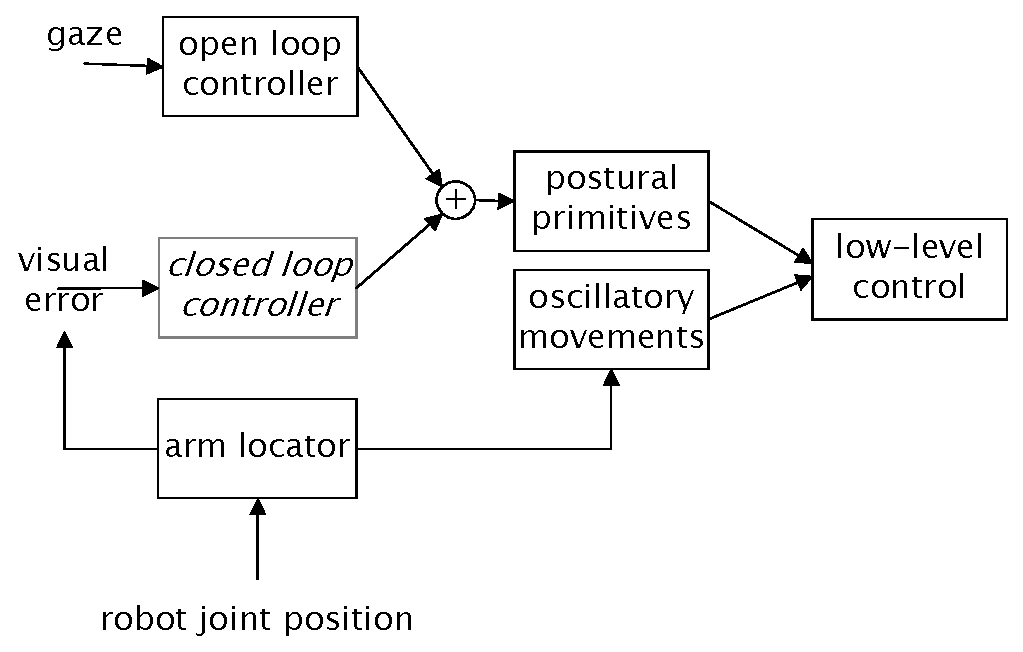
\includegraphics[width=\columnwidth]{control-flow.eps}
\caption{ 
\label{fig:control-flow}
%
  The controller.  Probably have to bring back text to describe this
  if we include this figure.
%
}
\end{center}
\end{figure}
\fi

\begin{figure}[tb]
\begin{center}
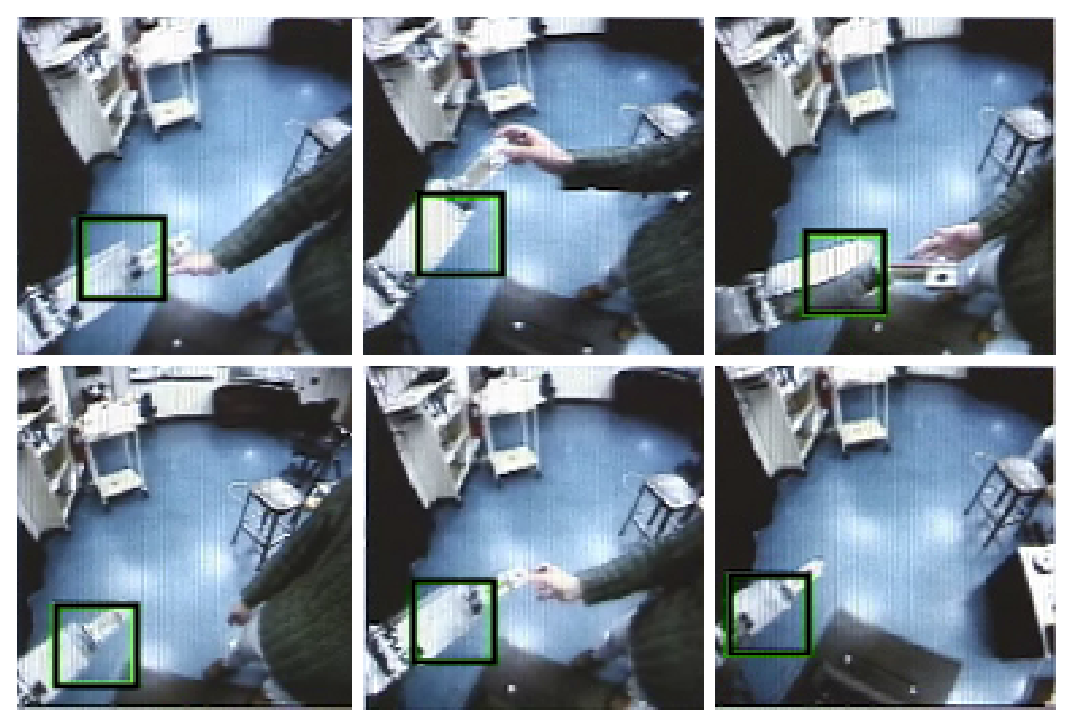
\includegraphics[width=6.0cm]{predict-position.eps}
%%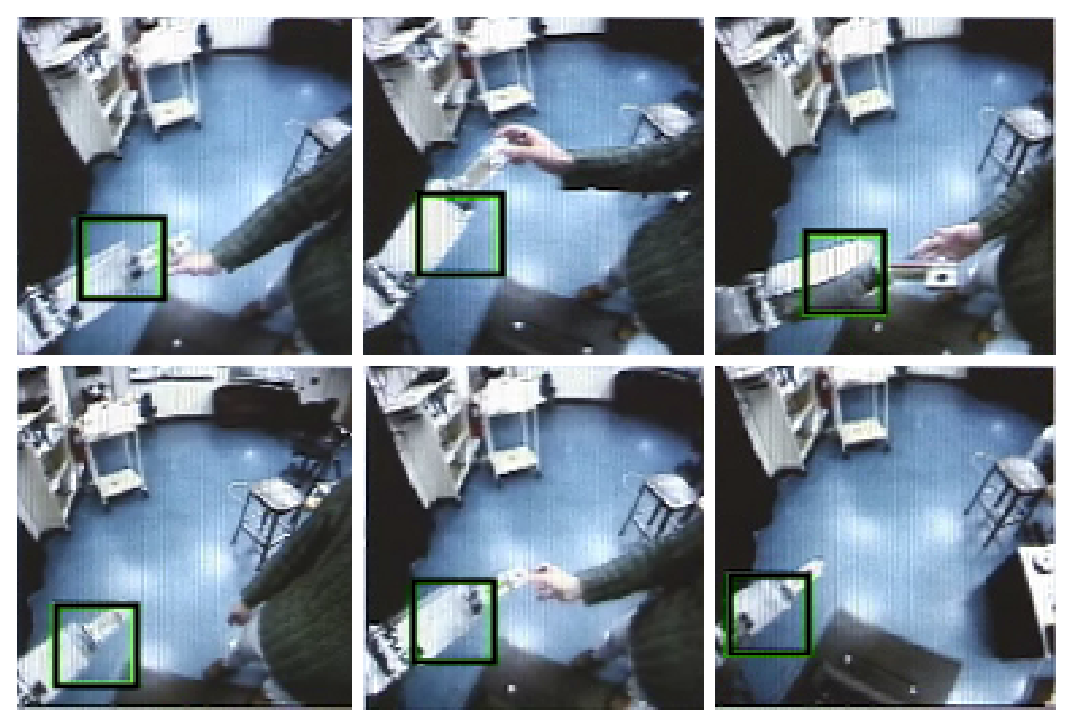
\includegraphics[width=\columnwidth]{predict-position.eps}
\caption{ 
\label{fig:predict-position}
%
Predicting the location of the arm in the image as the head and arm
change position. The rectangle represents the predicted position of
the arm using the map learned during a twenty-minute training run.
The predicted position just needs to be sufficiently accurate to
initialize a visual search for the exact position of the end-effector.
%
}
\end{center}
\end{figure}



\begin{figure}[tb]
\begin{center}
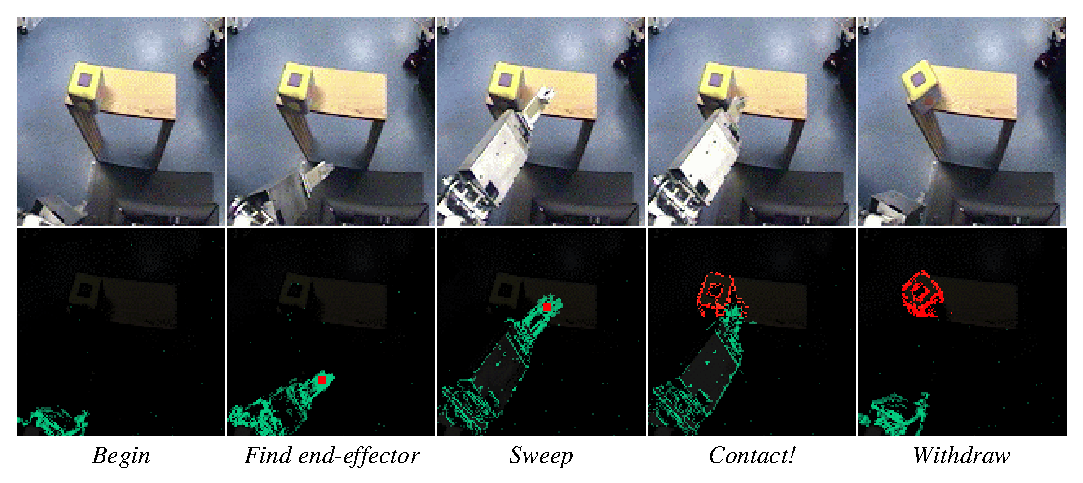
\includegraphics[width=\columnwidth]{poking-sequence.eps}

%%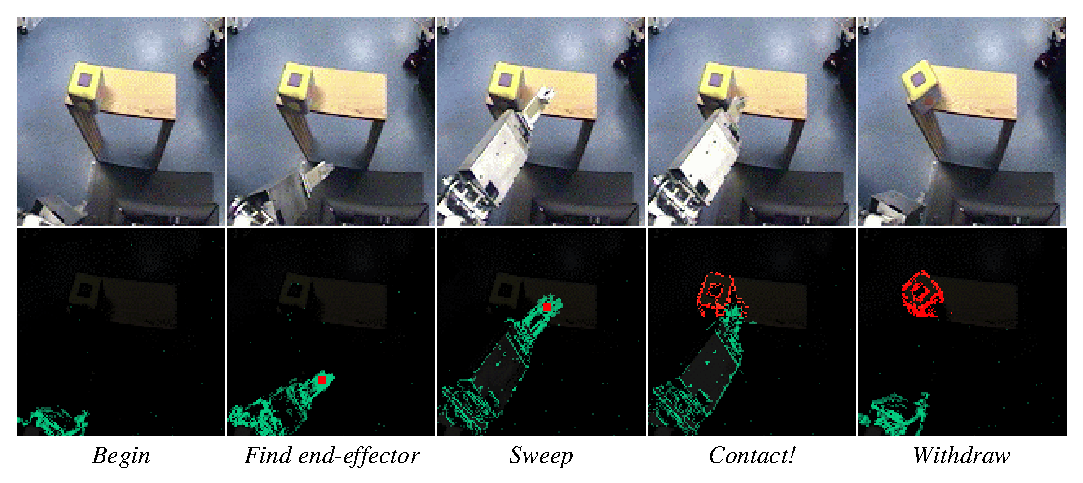
\includegraphics[width=\textwidth]{poking-sequence.eps}
%%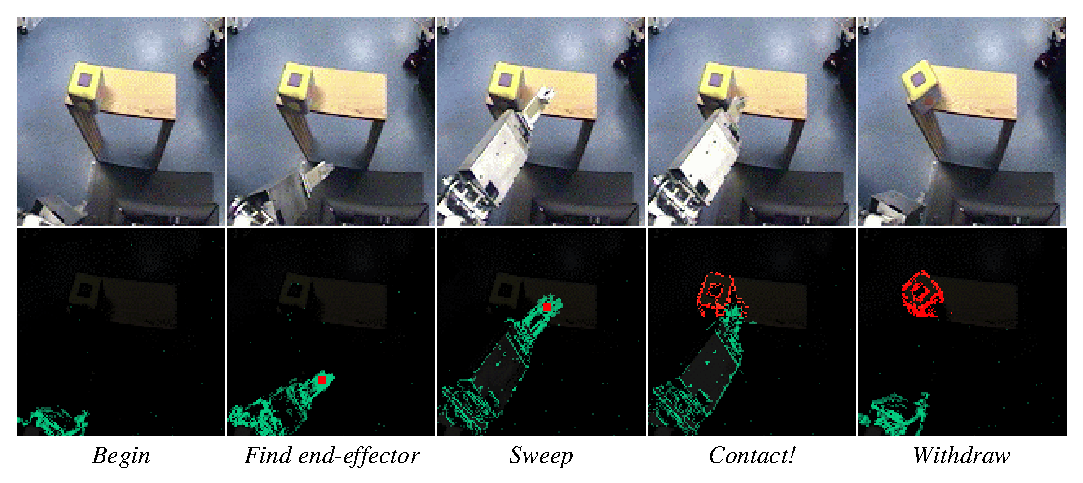
\includegraphics[width=14cm]{poking-sequence.eps}
\caption{ 
\label{fig:poking-sequence}
%
  The upper sequence shows an arm extending into a workspace, tapping
  an object, and retracting.  This is an exploratory mechanism for
  finding the boundaries of objects, and essentially requires the arm
  to collide with objects under normal operation, rather than as an
  occasional accident.  The lower sequence shows the shape
  identified from the tap using simple image differencing and flipper
  tracking.
%
}
\end{center}
\end{figure}



\section{Perceiving actions on objects}

Now that the robot knows something about its arm, it can start
to use it to explore its environment.
When the arm enters into contact with an object, one of several
outcomes are possible.  If the object is large, heavy, or otherwise
unyielding, motion of the arm may simply be resisted without any
visible effect.  Such objects are of little interest, except in their
role as obstacles, since the robot will not be able to manipulate
them.  But if the object is smaller, it is likely to move somewhat in
response to the nudge of the arm.  This movement will be temporally
correlated with the time of impact, and will be connected spatially to
the end-effector -- constraints that are not available in passive
scenarios~\cite{birchfield99depth}.  If the object is reasonably
rigid, and the movement has some component in parallel to the image
plane, the result is likely to be a flow field whose extent reflects
the physical boundaries of the object.  This visible response to
the robot's action can be used to refine its model of the object's
extent, which may be inaccurate.  For the example scene in
Figure~\ref{fig:setup-sequence} (a cube sitting on a table), the small
inner square on the cube's surface pattern might be selected as a
target.  The robot can certainly reach towards this target, but
grasping it would prove difficult without a correct estimate of the
object's physical extent.  In this section we show how the robot can
experimentally determine an object's extent using the same idea of
correlated motion used earlier to detect its own arm.

\subsubsection*{Making an impact}

Figure~\ref{fig:poking-sequence} shows how a ``poking'' movement can
be used to refine a target.  During this operation, the arm begins
by extending outwards from the resting position.  The end-effector (or
``flipper'') is localized as the arm sweeps rapidly outwards, using
the heuristic that it lies at the highest point of the region of optic
flow swept out by the arm in the image (the head orientation and
reaching trajectory are controlled so that this is true).  The arm is
driven outward into the neighborhood of the target which we wish to
define, stopping if an unexpected obstruction is reached.  If no
obstruction is met, the flipper makes a gentle sweep of the area
around the target.  This minimizes the opportunity for the motion of
the arm itself to cause confusion; the motion of the flipper is
bounded around the endpoint whose location we know from tracking
during the extension phase, and can be subtracted easily.  Flow not
connected to the end-effector can be ignored as a distractor.


The sequence shown in Figure~\ref{fig:poking-sequence} is about the
simplest case possible for segmenting the motion of the object, since most of the arm is stationary
when contact occurs.  In practice, we would rather have less
constraints on the motion of the arm, so we can approach the object
from any convenient direction.  We found that it was possible 
to attain this flexibility without losing the simplicity of object
segmentation that poking brings, by exploiting the unique
visual opportunity afforded by the moment of impact.


\ifverbose
For simplicity, the head is kept steady throughout the poking
operation, so that simple image differencing can be used to detect
motion at a higher resolution than optic flow.  Because a poking
operation currently always starts from the same location, the arm
is localized using a simple heuristic rather than the procedure described
in the previous section -- the first region of optic flow appearing
in the lower part of the robot's view when the reach begins
is assumed to be the arm.
\fi

\ifverbose
\begin{figure}[tbh]
\begin{center}
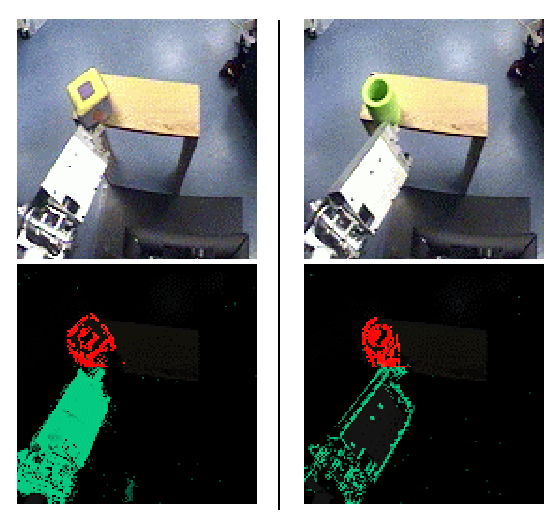
\includegraphics[width=\columnwidth]{cube-and-cylinder.eps}
\caption{ 
\label{fig:cube-and-cylinder}
%
  Poking can reveal a diffence in the shape of two objects without
  any prior knowledge of their appearance.
%
}
\end{center}
\end{figure}
\fi



\section{Detecting the point of collision}

Two components -- detecting the moment of impact, and extracting as 
much data as possible from the frames around it.

There are particular periods when the robot is attentive and fixating.
When this is so, it can detect visually when a collision occurs
between a moving object and a previously stationary object in view.
The principal task, then, is keep the motion of the moving object distinct
from that of the impacted object.

Brief introduction to image differencing and background subtraction.
Stationary camera assumption to facilitate pixel modeling.  Don't want
to keep head stationary, but can fixate for significant periods.

Image differencing is a very simple technique for detecting motion by
simply subtracting successive frames from a camera and looking for
pixel-level differences.  A moving object that has some contrast with
the background it is moving over will generate such differences.  Of
course, pixel differences can also be generated by changes in
illumination, cast shadows, computer monitors, movement of the camera
itself, etc.  A related technique called background modeling tries to
estimate the appearance of the fixed, stationary background of a 
scene, and then subtract the current view from the reference to 
detect new foreground.  While these techniques are not ideally
suited to a moving platform like our robot, they are short periods 
during which they can be useful.  In particular, when the robot is
fixating a target, we can do this.

Within the context of the robot fixating a target, we try to detect
the moment of impact precisely, so we can apply the (relatively) slow
segmentation optimization to a narrow interval of the video input and
maintain close to real-time performance.  A moving manipulator
colliding with an object will accelerate it, if it is not too massive.
If the object is rigid, the motion of the manipulator will be transmitted 
through it.  This transmission can be detected as a spreading motion
that is not plausibly generated by the manipulator itself.

Some assumptions that may fail: object not too heavy; object at least
semi-rigid; manipulator not moving above a certain speed; manipulator
not casting shadows on the object itself.  When the robot is poking the
object itself, it can control some of this.  If the object iself is
troublesome, then we potentially diagnose this, or just ignore it.

%%We are relying on some facts about optic flow.  When an object is ...

\begin{figure}[tbh]
  \begin{center}
    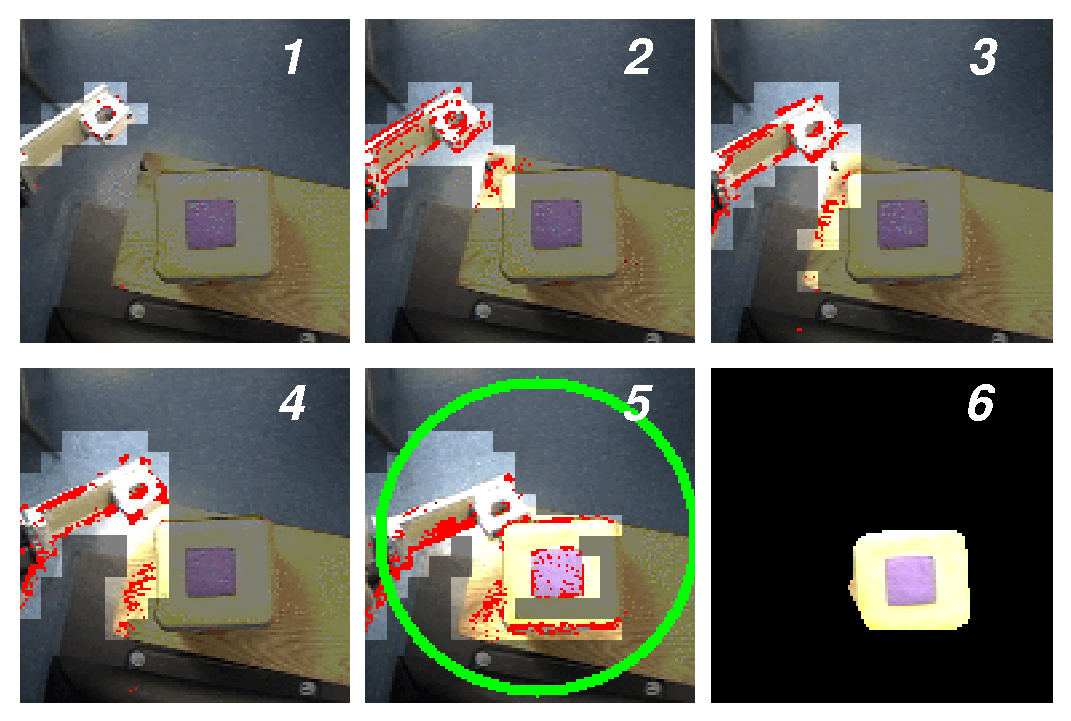
\includegraphics[width=12cm]{collision-detail}
  \end{center}
  \caption{
    The moment of impact is detected visually by the
    sudden expansion of motion away from the arm.  Motion before and
    after contact is compared to gather information for segmentation.
}
\end{figure}



\subsubsection*{An operational definition of objecthood}

The poking operation gives clear results for a rigid object that is
free to move.  What happens for non-rigid objects and objects that are
attached to other objects?  Here the results of poking are likely to
be more complicated to interpret -- but in a sense this is a good
sign, since it is in just such cases that the idea of an object
becomes less well-defined.  Poking has the potential to offer an
operational theory of ``objecthood'' that is more tractable than a
vision-only approach might give, and which cleaves better to the true
nature of physical assemblages.  The idea of a physical object is
rarely completely coherent, since it depends on where you draw its
boundary and that may well be task-dependent.  Poking allows us to
determine the boundary around a mass that moves together when
disturbed, which is exactly what we need to know for manipulation.  As
an operational definition of object, this has the attractive property
of breaking down into ambiguity in the right circumstances~-- such as
for large interconnected messes, floppy formless ones, liquids, and so
on.  Poking also gives the robot the opportunity
to collect many views of a single object, and so we can hope to deal
with recognizing objects like the cube shown in
Figure~\ref{fig:sample-results}, which look different from every side.


\begin{figure}[tbh]
  \centerline{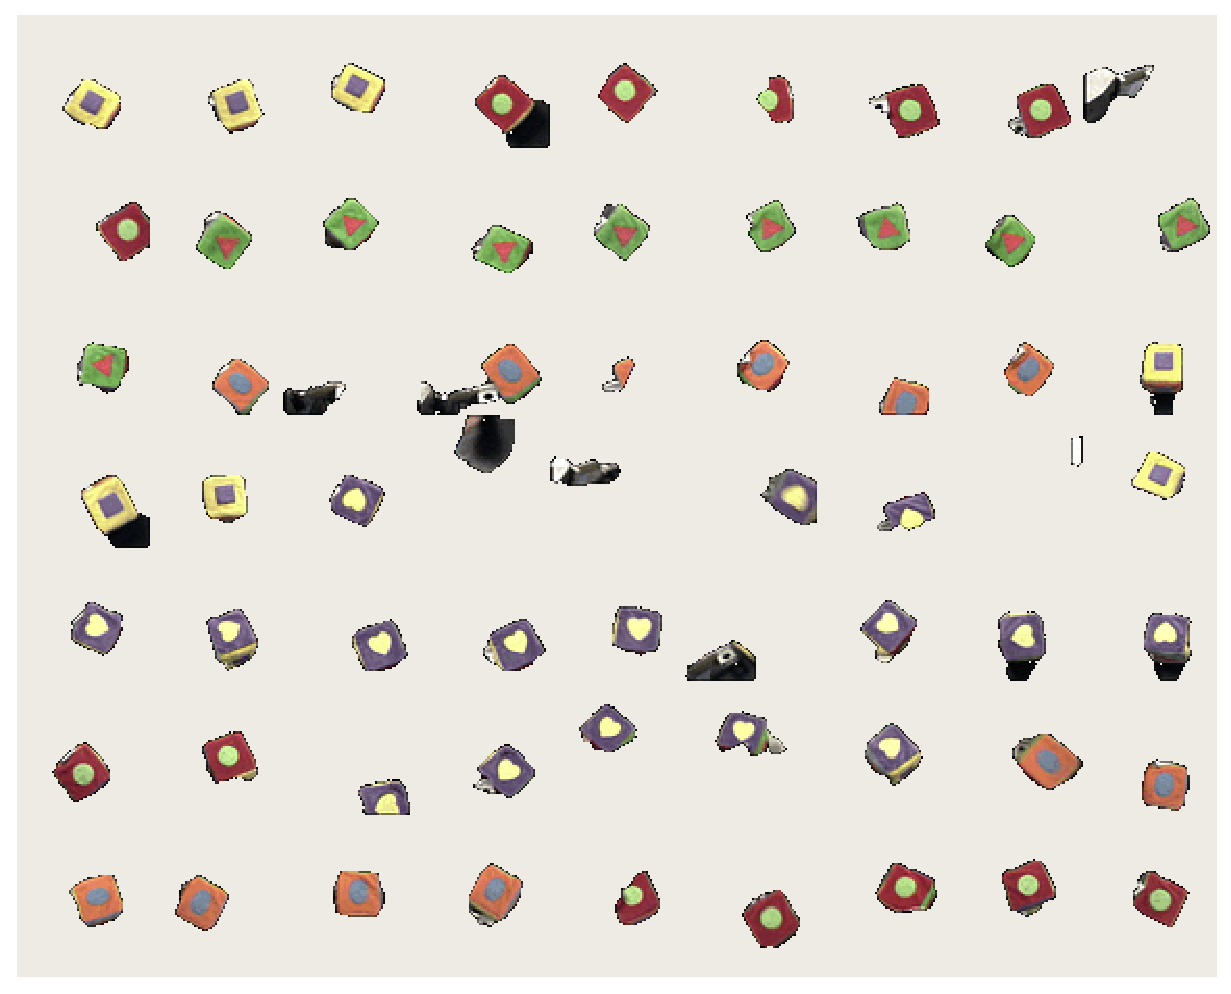
\includegraphics[width=9cm]{experiment-montage}}
  \caption{ 
  \label{fig:sample-results}
Results of a training session, where a toy cube was
  repeatedly offered to the robot for poking.  Each image of the cube
  corresponds to the segmentation found for it during a single poke.
  The most common failure mode is inclusion of the robot arm in the
  segmentation.  
}
\end{figure}




\section{Developing mirror neurons?}

\begin{figure}[tb]
\begin{center}
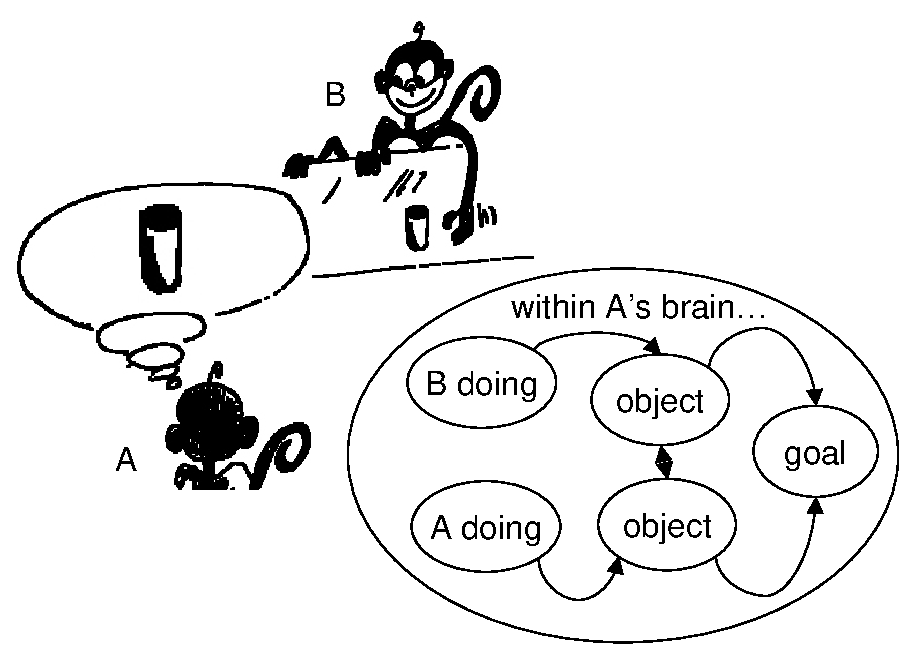
\includegraphics[width=\columnwidth]{mirror-monkey.eps}
\caption{ 
\label{fig:mirror-monkey}
%
Mirror neurons and causality: from the observer's point
of view (A), understanding B's action means mapping it onto the
observer's own
motor repertoire. If the causal chain leading to the goal is already
in place (lower branch of the graph) then the acquisition of a
mirror neuron for this particular action/object is a matter of
building and linking the upper part of the chain to the lower one.
There are various opportunities to reinforce this link either at the object
level, at the goal level or both. 
%%Developmentally we can explain
%%mirror neurons only if we take into account another class of neurons
%%(called canonical) which in practice describes the lower branch of the
%%graph.
%
}
\end{center}
\end{figure}

\ifverbose
The latest instantiation of the ``general principle'' we would like to
dwell upon is related to mirror neurons. It turns out that the causal
chain here is more compliceted. This requires a more complicated
structure to support it.
\fi

Poking moves us one step outwards on a causal chain away from the
robot and into the world, and gives a simple experimental procedure
for segmenting objects.  There are many possible elaborations of this
method (some are mentioned in the conclusions), all of which lead to a
vision system that is tuned to acquiring data about an object by
seeing it manipulated by the robot.  An interesting question then is
whether the system could extract useful information from seeing an
object manipulated by someone else.  In the case of poking, the robot
needs to be able to estimate the moment of contact and to track the arm
sufficiently well to distinguish it from the object being poked.  We
are interested in how the robot might learn to do this.  One approach
is to chain outwards from an object the robot has poked.  If someone
else moves the object, we can reverse the logic used in poking --
where the motion of the manipulator identified the object -- and
identify a foreign manipulator through its effect on the object.
Poking is an ideal testbed for future work on this, since it is much
simpler than full-blown object manipulation and would only require a
very simple model of the foreign manipulator to work.

There is considerable precedent in the biological literature for a
strong connection between viewing object manipulation performed by
either oneself or another \cite{wohlsclager02human}. Also
the role of object in the understanding of action performed by others
has been investigated~\cite{woodward98infants}. In a series of
experiments Woodward and colleagues elucidated the contribution that
seeing an object makes for 5, 6, and 9 month old infants. They
provided evidence that the object and the goal-directness of the
action represent an important component in the understanding of the
intentions of others.

At the neural level, we already mentioned the presence of neurons in
F5 that have a very specific response when an object is either fixated
or manipulated (canonical neurons). Grossly simplifying, we might
think of canonical neurons as an association table of
grasp/manipulation (action) types with object (vision) types.

F5 also contains mirror neurons. These neurons, as we described
before, respond when either watching somebody else performing a
manipulative action or when actually manipulating an object. They can
be thought of as a second-level association map which links together
the observation of a manipulative action performed by somebody else
with the neural representation of one's own action.

The question of whether a mirror-like representation can be
autonomously developed by the robot (or a human for that matter) can
then be answered. The association map can be constructed by
identifying when the goal and the object are the same irrespective of
who is the actor. Actions that lead to the same consequences are thus
part of the same equivalence class.  This is exactly what mirror neurons
represent.


\ifverbose
There is considerable precedent in the literature for a strong
connection between viewing object manipulation performed by either
oneself or another \cite{wohlsclager02human}.  As we already mentioned
F5 contains a class of neurons called canonical neurons that have a
very specific response when an object is being either manipulated or
fixated.  Grossly simplifying, we might think of canonical neurons as
an association table of grasp/manipulation (action) types with object
(vision) types.  Another class of neurons called ``mirror neurons''
can then be thought of as a second-level association map which links
together the observation of a manipulative action performed by
somebody else with the neural representation of one's own action.
\fi

Figure~\ref{fig:mirror-monkey} shows this causal chain in action.
There are a series of interesting behaviors that can be realized based
on mirror neurons. Mimicry is an obvious application, since it
requires just this type of mapping between other and self in terms of
motor actions.  Another important application is the prediction of
future behavior from current actions, or even inverting the causal
relation to find the action that most likely will get to the desired
consequence.

\ifverbose

for example, by observing the part of an action the robot or the
bioagent can come out with suitable expectations of the consequences
of that action. On the other hand, the inverse behavior can also be
foreseen. The latter account to inverting the causal relation and
getting the action that most likely will get to the desired
consequence.

It might be argued that we need a two stages procedure to learn a
mirror representation, where we first learn ``something'' and only
subsequently we ``understand'' other people's behavior. The actual
developmental course might not be such artificially staged. A slight
advantage must be given though to the initial step of self-learning,
the undestanding comes later.


This set of associations can be learnt autonomously (by a robot for
example) simply by a trial and error procedure and possibly with a
reinforcing signal to tell when a given grasp/manipulatory gesture was
successful if applied to a particular object.

We should not probably think of this association as describing in
detail the object being manipulated visually. Perhaps only features
relevant to manipulation are stored (e.g. size, orientation in space).
This representation is a ``pragmatic'' one describing only those
properties of objects are needed to apply a particular set of actions
to them. Affordances are a good psychological analogue of F5
canonical neurons.
\fi


\ifverbose
How does this relate to causation?  The two situations in some sense
share the same goal, and more practically share the same object.  The
whole procedure assumes a basic discrimination of size and shape of
objects (not necessarily categorization in traditional sense), and the
exploitation of the visual information to the understanding of the
grasp type. In some cases though the goal might be unambiguous, e.g. a
needle is very unlikely grasped with a full palm grasp, as well as a
box is not grasped with a pinch grip. These are the most informative
allowing for the best discrimination of action type from the visual
perspective.
\fi

\ifverbose
The definition of imitation we gave here implicitly focus on imitating
the goal rather than the precise trajectory. This automatically takes
into account any difference in body structure between the actor and
the observer.

Of course, manipulation as in poking can lead to a better
understanding of the physical properties of objects not directly
amenable to visual exploration such as mass, roughness, softness, etc.
\fi

\ifverbose
\begin{figure}[tbh]
\begin{center}
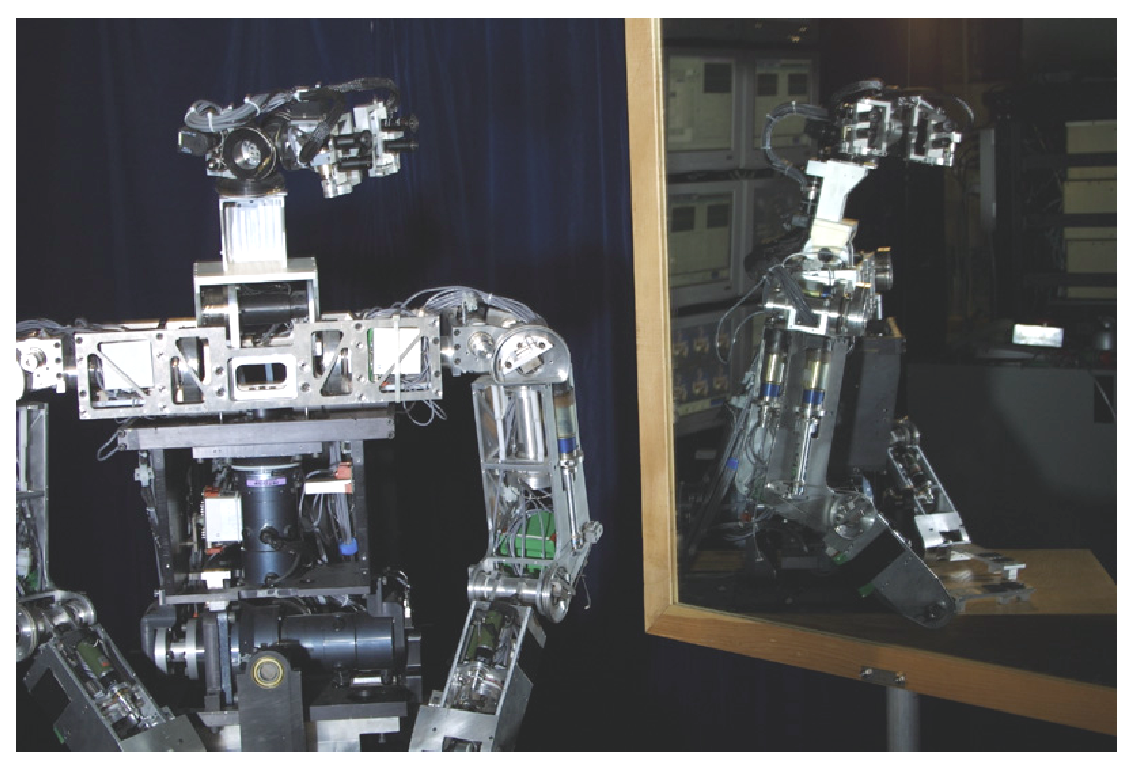
\includegraphics[width=\columnwidth]{mirror-cog.eps}
\caption{ 
\label{fig:mirror-cog}
%
The ultimate goal of this work is for our robot to follow chains of
causation outwards from its own simple body into the complex world.
%
}
\end{center}
\end{figure}
\fi



\section{Discussion and Conclusions}

In this paper, we showed how causality can be probed at different
levels by the robot.  Initially the environment was the body of the
robot itself, then later a carefully circumscribed interaction with
the outside world.  This is reminiscent of Piaget's distinction
between primary and secondary circular
reactions~\cite{ginsburg78piaget}.  Objects are central to interacting
with the outside world.  We raised the issue of how an agent can
autonomously acquire a working definition of objects. 

In computer vision there is much to be gained by bringing a
manipulator into the equation.  Many variants and extensions to the
experimental ``poking'' strategy explored here are possible.  For
example, a robot might try to move an arm around {\em behind} the
object.  As the arm moves behind the object, it reveals its occluding
boundary.  This is a precursor to visually extracting shape
information while actually manipulating an object, which is more
complex since the object is also being moved and partially occluded by
the manipulator.  Another possible strategy that could be adopted as a
last resort for a confusing object might be to simply hit it firmly,
in the hopes of moving it some distance and potentially overcoming
local, accidental visual ambiguity.  Obviously this strategy cannot
always be used!  But there is plenty of room to be creative here.
%
%
\ifrev
%
There are also limitations in our current implementation that could
usefully be addressed.
%
The robot itself is not mobile, so its workspace is limited.  
%
There are also many constraints on the arm that make fine 
motor control impossible -- it cannot maintain all reachable 
poses indefinitely, and there is significant noise and some 
hysteresis in its analog sensors.
%
The robot will only attempt to reach towards a target that is 
actually accessible to its arm -- not too close, not too far, 
as determined using visual disparity.  In practice, this 
means that the ideal workspace is a table in front of the 
robot, and the motor control of the robot has been 
specifically tuned to work well in that situation.
%
A simple attention system and tracking mechanism are used to 
bring the robot's attention to a target.  This phase can fail 
if the robot gets distracted by some more salient (but 
unreachable) part of the scene.
%
Objects that move together are not individually segmented.
%
And segmentation does not always succeed, due to shadows,
or strong nearby edges.
%
\fi

The robotic experiments support the view that reaching, grasping, and recognition
can be learned by following a particular ontogenetic pathway without the
intervention of an external teacher.
This pathway is consistent with and inspired by what is
known of this process in biological systems (primates/mammals).
%although this evidence is rather sparse.
%
We have endeavored to build from as few innate components as possible, to
elucidate the visual and motor challenges faced by a learning robot rather
than simply solving them by fiat.
%
%There is relatively little evidence to work with, but it is at least clear that the 
%sequence of events leading to object manipulation/recognition cannot take
%an arbitrary form unless we assume that some/many of its components are innate.
Although newborns show amazing abilities \cite{spelke-2000} such as early imitation 
\cite{meltzoff-moore-1977}, face detection, etc, there is also evidence 
that the maturation of the brain is far from complete at birth and
complex perceptual abilities require a long time to emerge \cite{kovacs00human}.
%
We have given a simple existence proof that object segmentation,
recognition and localization can develop without any prior knowledge
of visual appearance.  We have also shown that, without any prior
knowledge of the human form, the robot can identify episodes when a
human is manipulating objects that are familiar to the robot purely by
the operational similarity of the human arm and its own manipulator in
this situation.  We believe such demonstrations are important both in
their own right, and in their elucidation of a concrete series of
steps that lead to a desired behavior.  This may serve a useful
reference point from which to investigate the biological solution to
the same problem -- although it can't provide the answers, it can at
least suggests useful questions.

%
%This is important, since segmentation and recognition as usually expressed 
%suffer from a chicken-and-egg problem, where views of an object must be
%segmented before its appearance can be learned...

%We cannot claim that this is the only possible view but it is certainly one worth
%investigating. Rephrasing Berkeley we can say:
%\begin{quote}
%...objects can only be known by
%\emph{action}. Vision is subject to illusions, 
%which arise from \emph{many different} problems...
%\end{quote}
%that AI guys know far too well

%Could relate some of this to the embodied intelligence ideas
%of Brooks... particularly the working hypothesis.



% thanks to many people...


\section*{Acknowledgements}

Many people have contributed to developing the Cog platform
\cite{brooks99cog}.  This work benefited from discussions with Charles Kemp
and Giulio Sandini, and the perceptive comments of reviewers.  
Funds for this project were provided by DARPA 
%%as
%%part of the ``Natural Tasking of Robots Based on Human Interaction
%%Cues'' project under 
(contract number DABT 63-00-C-10102), and by the
Nippon Telegraph and Telephone Corporation as part of the NTT/MIT
Collaboration Agreement.



% and the bibliography:

\newpage

%%\bibliography{abbreviations,biblio}
% **** PUT YOUR OWN BIBLIOGRAPHY FILES IN HERE ****

\bibliographystyle{plain}

\bibliography{vision}



\section{Extras}


\begin{figure}[tbh]
  \begin{center}
    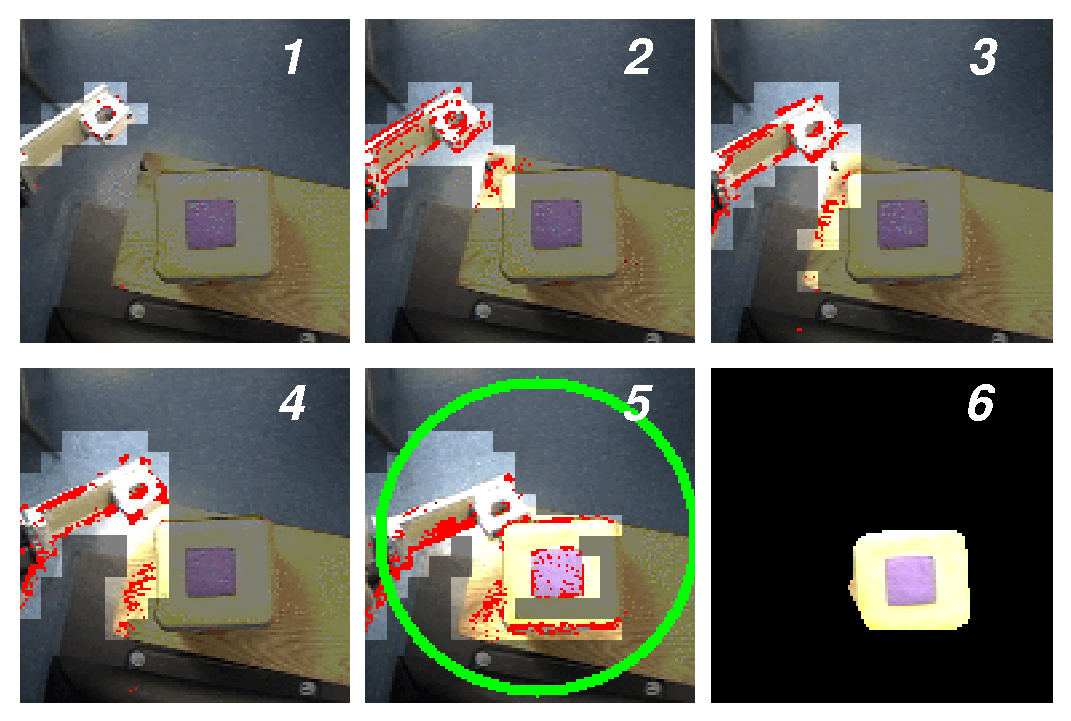
\includegraphics[width=2in]{collision-detail}
    \hspace{1in}
    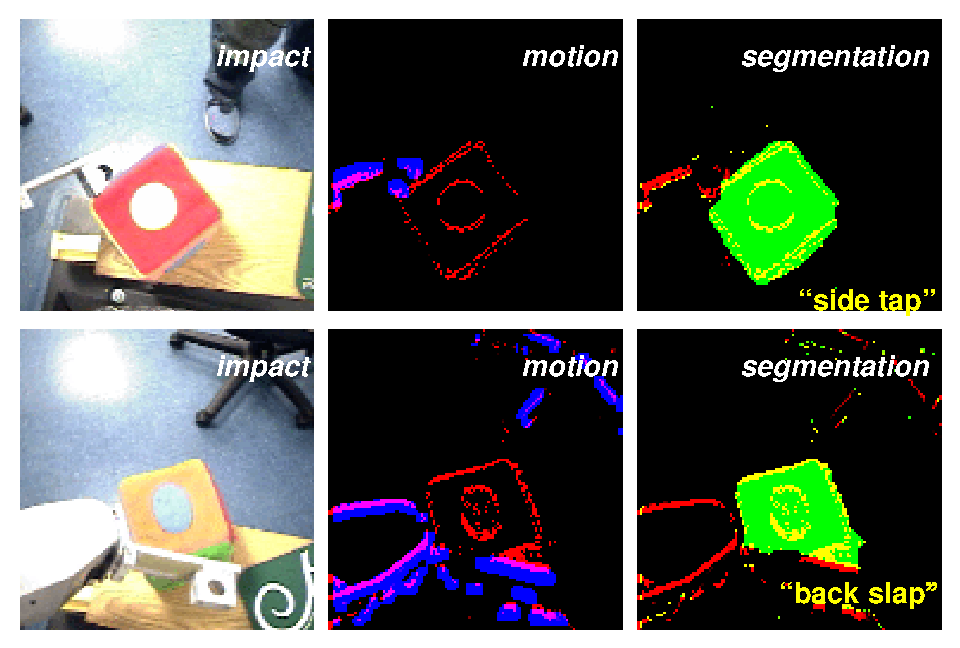
\includegraphics[width=2in]{segmentation-detail}
  \end{center}
  \caption{Part of the process}
\end{figure}

\begin{figure}[tbh]
  \centerline{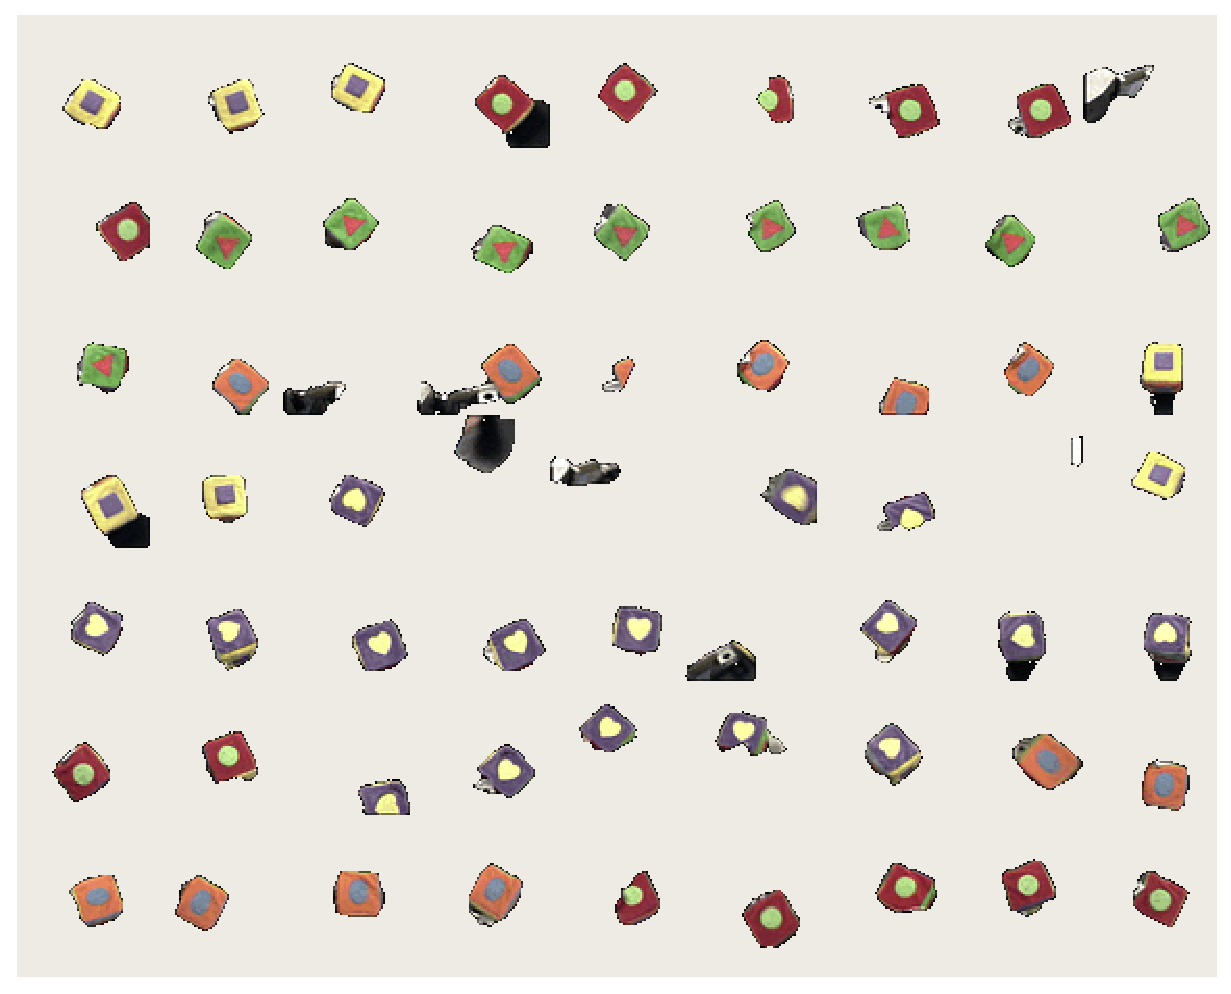
\includegraphics[width=2.5in]{experiment-montage}}
  \caption{Sample results}
  \label{fig:sample-results}
\end{figure}

\begin{figure}[tbh]
  \centerline{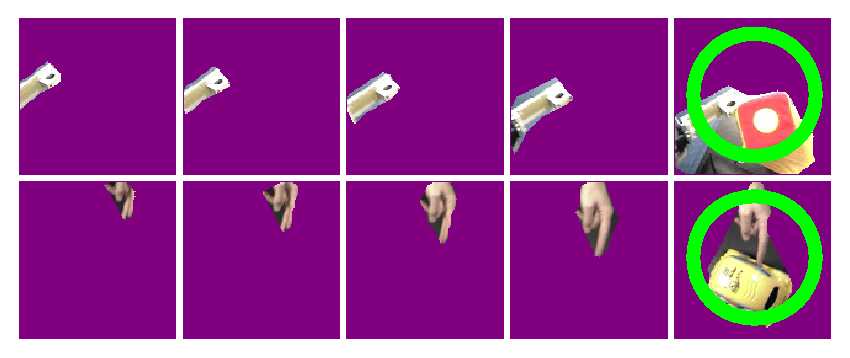
\includegraphics[width=2.5in]{manipulator-segment}}
  \caption{Segmenting the manipulator} 
  \label{fig:manipulator}
\end{figure}

\begin{figure}[tbh]
  \centerline{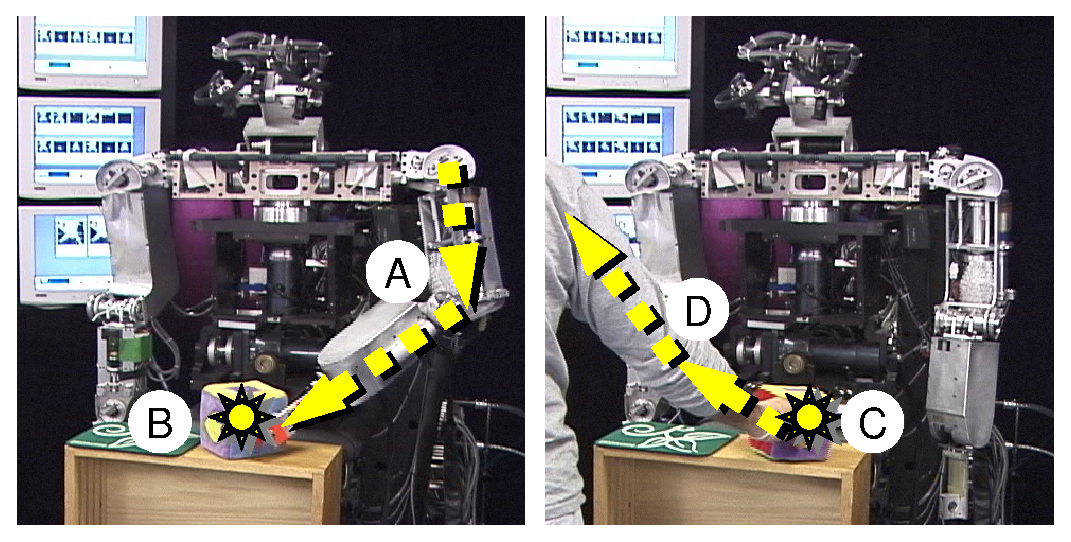
\includegraphics[width=2.5in]{tracing_causes}}
  \caption{foo} 
  %%\label{fig:foo}
\end{figure}


\begin{figure}[tbh]
  \centerline{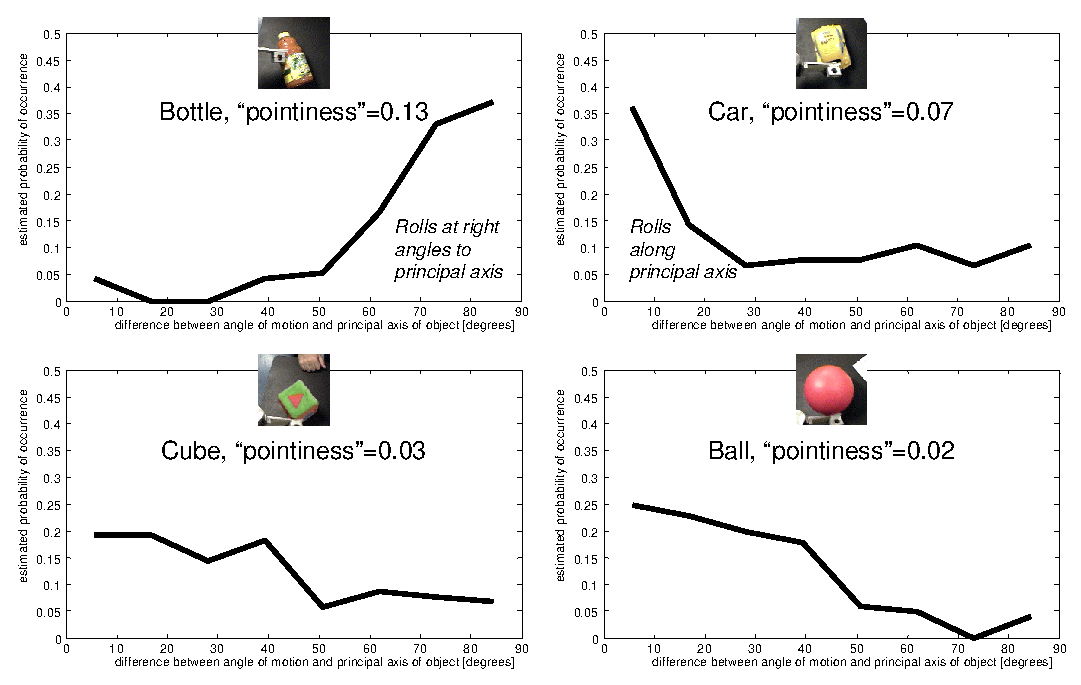
\includegraphics[width=2.5in]{rolling-graphs}}
  \caption{foo} 
  %%\label{fig:foo}
\end{figure}




\newpage

\listoftables

\newpage

\listoffigures




%% 
\section{Closing the loop}

%% rolling experiment

Poking is sufficient to explore some very simple affordances of
objects, such as rolling, toppling, breaking etc.  We explore the
rolling affordance with the four objects shown in
Figure~\ref{fig:rolling-motivate}.  Each of the objects rolls in a
different way, which the robot can learn about and exploit.

\begin{figure}[tbh]
  \centerline{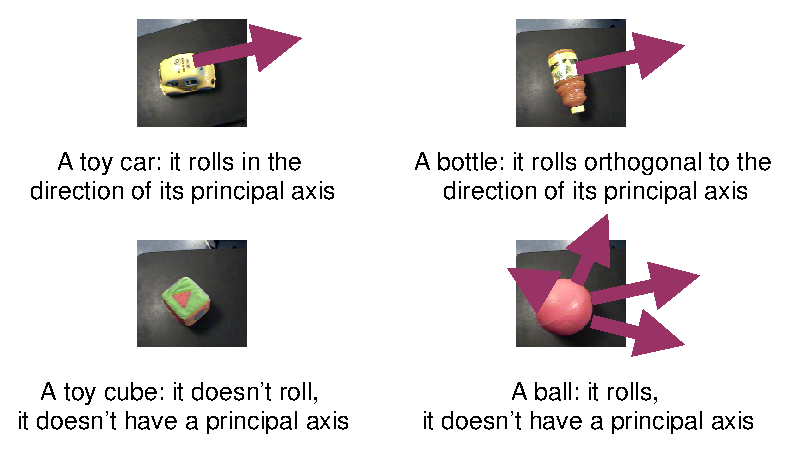
\includegraphics[width=12cm]{rolling-motivate}}
  \caption{
%
    Different objects roll in different ways.  A toy car rolls
    forward, a bottle rolls on its side, a sphere rolls in any
    direction, and a cube doesn't really roll at all.
%
} 
  \label{fig:rolling-motivate}
\end{figure}

\begin{figure}[tbh]
  \centerline{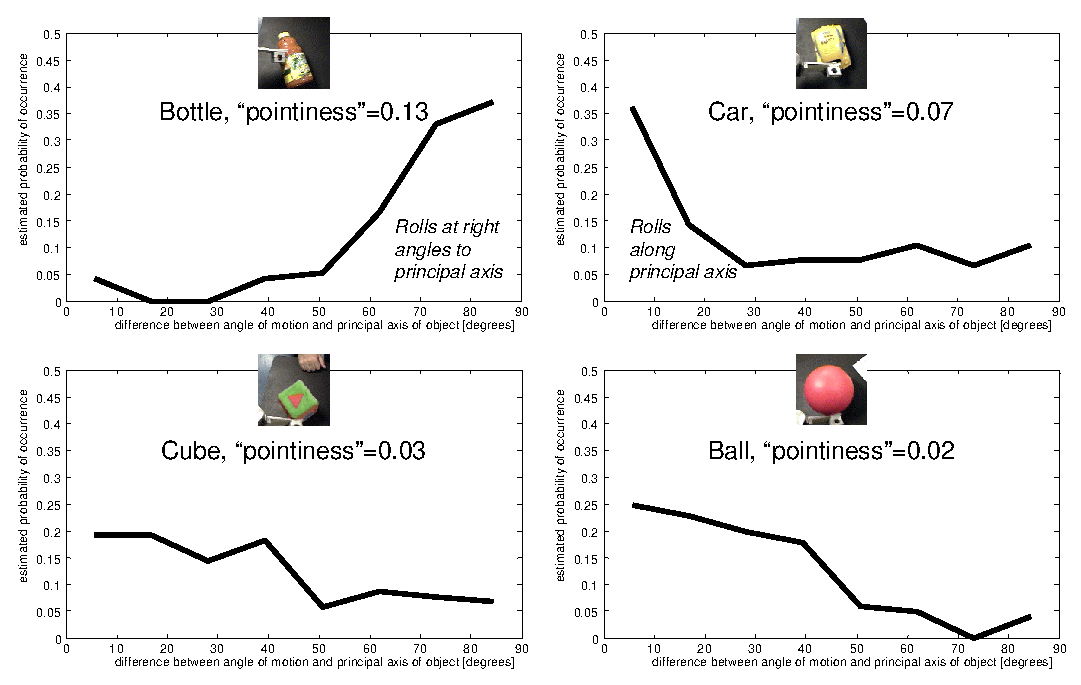
\includegraphics[width=12cm]{rolling-graphs}}
  \caption{
%
  The robot relates the direction an object moves in with the
  direction of its principal axis.  For a car, there is a clear
  tendency to roll in the direction of the principal axis.
  A bottle has a clear tendency to roll towards its side.
  Cars and spheres have no clear principal axis so, whether they
  roll or not, there is nothing to say.
%
} 
  \label{fig:rolling-graphs}
\end{figure}

The final behavior of the robot after training is: human presents an
object, makes it roll.  Presents the same object, perhaps in another
orientation, and the robot pushes it in the right direction to make it
roll.  If the human hits the object in a non-canonical direction,
so will the robot.  This serves to demonstrate the full loop of 
perception and action.






\end{document}

% and never mind LaTeX's hysterical warnings about missing fonts... everything's fine!
